\documentclass[twoside]{book}

% Packages required by doxygen
\usepackage{calc}
\usepackage{doxygen}
\usepackage{graphicx}
\usepackage[utf8]{inputenc}
\usepackage{makeidx}
\usepackage{multicol}
\usepackage{multirow}
\usepackage{textcomp}
\usepackage[table]{xcolor}

% Font selection
\usepackage[T1]{fontenc}
\usepackage{mathptmx}
\usepackage[scaled=.90]{helvet}
\usepackage{courier}
\usepackage{amssymb}
\usepackage{sectsty}
\renewcommand{\familydefault}{\sfdefault}
\allsectionsfont{%
  \fontseries{bc}\selectfont%
  \color{darkgray}%
}
\renewcommand{\DoxyLabelFont}{%
  \fontseries{bc}\selectfont%
  \color{darkgray}%
}

% Page & text layout
\usepackage{geometry}
\geometry{%
  a4paper,%
  top=2.5cm,%
  bottom=2.5cm,%
  left=2.5cm,%
  right=2.5cm%
}
\tolerance=750
\hfuzz=15pt
\hbadness=750
\setlength{\emergencystretch}{15pt}
\setlength{\parindent}{0cm}
\setlength{\parskip}{0.2cm}
\makeatletter
\renewcommand{\paragraph}{%
  \@startsection{paragraph}{4}{0ex}{-1.0ex}{1.0ex}{%
    \normalfont\normalsize\bfseries\SS@parafont%
  }%
}
\renewcommand{\subparagraph}{%
  \@startsection{subparagraph}{5}{0ex}{-1.0ex}{1.0ex}{%
    \normalfont\normalsize\bfseries\SS@subparafont%
  }%
}
\makeatother

% Headers & footers
\usepackage{fancyhdr}
\pagestyle{fancyplain}
\fancyhead[LE]{\fancyplain{}{\bfseries\thepage}}
\fancyhead[CE]{\fancyplain{}{}}
\fancyhead[RE]{\fancyplain{}{\bfseries\leftmark}}
\fancyhead[LO]{\fancyplain{}{\bfseries\rightmark}}
\fancyhead[CO]{\fancyplain{}{}}
\fancyhead[RO]{\fancyplain{}{\bfseries\thepage}}
\fancyfoot[LE]{\fancyplain{}{}}
\fancyfoot[CE]{\fancyplain{}{}}
\fancyfoot[RE]{\fancyplain{}{\bfseries\scriptsize Generated on Sat May 21 2016 22\-:33\-:28 for Jerry -\/ Chess G\-U\-I by Doxygen }}
\fancyfoot[LO]{\fancyplain{}{\bfseries\scriptsize Generated on Sat May 21 2016 22\-:33\-:28 for Jerry -\/ Chess G\-U\-I by Doxygen }}
\fancyfoot[CO]{\fancyplain{}{}}
\fancyfoot[RO]{\fancyplain{}{}}
\renewcommand{\footrulewidth}{0.4pt}
\renewcommand{\chaptermark}[1]{%
  \markboth{#1}{}%
}
\renewcommand{\sectionmark}[1]{%
  \markright{\thesection\ #1}%
}

% Indices & bibliography
\usepackage{natbib}
\usepackage[titles]{tocloft}
\setcounter{tocdepth}{3}
\setcounter{secnumdepth}{5}
\makeindex

% Hyperlinks (required, but should be loaded last)
\usepackage{ifpdf}
\ifpdf
  \usepackage[pdftex,pagebackref=true]{hyperref}
\else
  \usepackage[ps2pdf,pagebackref=true]{hyperref}
\fi
\hypersetup{%
  colorlinks=true,%
  linkcolor=blue,%
  citecolor=blue,%
  unicode%
}

% Custom commands
\newcommand{\clearemptydoublepage}{%
  \newpage{\pagestyle{empty}\cleardoublepage}%
}


%===== C O N T E N T S =====

\begin{document}

% Titlepage & ToC
\hypersetup{pageanchor=false}
\pagenumbering{roman}
\begin{titlepage}
\vspace*{7cm}
\begin{center}%
{\Large Jerry -\/ Chess G\-U\-I \\[1ex]\large 3 }\\
\vspace*{1cm}
{\large Generated by Doxygen 1.8.6}\\
\vspace*{0.5cm}
{\small Sat May 21 2016 22:33:28}\\
\end{center}
\end{titlepage}
\clearemptydoublepage
\tableofcontents
\clearemptydoublepage
\pagenumbering{arabic}
\hypersetup{pageanchor=true}

%--- Begin generated contents ---
\chapter{Hierarchical Index}
\section{Class Hierarchy}
This inheritance list is sorted roughly, but not completely, alphabetically\-:\begin{DoxyCompactList}
\item \contentsline{section}{chess\-:\-:Arrow}{\pageref{structchess_1_1Arrow}}{}
\item \contentsline{section}{chess\-:\-:Board}{\pageref{classchess_1_1Board}}{}
\item \contentsline{section}{chess\-:\-:Colored\-Field}{\pageref{structchess_1_1ColoredField}}{}
\item \contentsline{section}{chess\-:\-:Game}{\pageref{classchess_1_1Game}}{}
\item \contentsline{section}{chess\-:\-:Game\-Node}{\pageref{classchess_1_1GameNode}}{}
\item \contentsline{section}{chess\-:\-:Gui\-Printer}{\pageref{classchess_1_1GuiPrinter}}{}
\item \contentsline{section}{chess\-:\-:Header\-Offset}{\pageref{structchess_1_1HeaderOffset}}{}
\item \contentsline{section}{chess\-:\-:Move}{\pageref{classchess_1_1Move}}{}
\item \contentsline{section}{chess\-:\-:Pgn\-Printer}{\pageref{classchess_1_1PgnPrinter}}{}
\item \contentsline{section}{chess\-:\-:Pgn\-Reader}{\pageref{classchess_1_1PgnReader}}{}
\item Q\-Main\-Window\begin{DoxyCompactList}
\item \contentsline{section}{Main\-Window}{\pageref{classMainWindow}}{}
\end{DoxyCompactList}
\item Q\-Object\begin{DoxyCompactList}
\item \contentsline{section}{chess\-:\-:Func\-T}{\pageref{classchess_1_1FuncT}}{}
\end{DoxyCompactList}
\end{DoxyCompactList}

\chapter{Class Index}
\section{Class List}
Here are the classes, structs, unions and interfaces with brief descriptions\-:\begin{DoxyCompactList}
\item\contentsline{section}{\hyperlink{structchess_1_1Arrow}{chess\-::\-Arrow} }{\pageref{structchess_1_1Arrow}}{}
\item\contentsline{section}{\hyperlink{classchess_1_1Board}{chess\-::\-Board} }{\pageref{classchess_1_1Board}}{}
\item\contentsline{section}{\hyperlink{structchess_1_1ColoredField}{chess\-::\-Colored\-Field} }{\pageref{structchess_1_1ColoredField}}{}
\item\contentsline{section}{\hyperlink{classchess_1_1FuncT}{chess\-::\-Func\-T} }{\pageref{classchess_1_1FuncT}}{}
\item\contentsline{section}{\hyperlink{classchess_1_1Game}{chess\-::\-Game} }{\pageref{classchess_1_1Game}}{}
\item\contentsline{section}{\hyperlink{classchess_1_1GameNode}{chess\-::\-Game\-Node} }{\pageref{classchess_1_1GameNode}}{}
\item\contentsline{section}{\hyperlink{classchess_1_1GuiPrinter}{chess\-::\-Gui\-Printer} }{\pageref{classchess_1_1GuiPrinter}}{}
\item\contentsline{section}{\hyperlink{structchess_1_1HeaderOffset}{chess\-::\-Header\-Offset} }{\pageref{structchess_1_1HeaderOffset}}{}
\item\contentsline{section}{\hyperlink{classMainWindow}{Main\-Window} }{\pageref{classMainWindow}}{}
\item\contentsline{section}{\hyperlink{classchess_1_1Move}{chess\-::\-Move} }{\pageref{classchess_1_1Move}}{}
\item\contentsline{section}{\hyperlink{classchess_1_1PgnPrinter}{chess\-::\-Pgn\-Printer} }{\pageref{classchess_1_1PgnPrinter}}{}
\item\contentsline{section}{\hyperlink{classchess_1_1PgnReader}{chess\-::\-Pgn\-Reader} }{\pageref{classchess_1_1PgnReader}}{}
\end{DoxyCompactList}

\chapter{Class Documentation}
\hypertarget{structchess_1_1Arrow}{\section{chess\-:\-:Arrow Struct Reference}
\label{structchess_1_1Arrow}\index{chess\-::\-Arrow@{chess\-::\-Arrow}}
}
\subsection*{Public Attributes}
\begin{DoxyCompactItemize}
\item 
\hypertarget{structchess_1_1Arrow_a9c5c8fb47db6240ad6b01710ec1873da}{Q\-Point {\bfseries from}}\label{structchess_1_1Arrow_a9c5c8fb47db6240ad6b01710ec1873da}

\item 
\hypertarget{structchess_1_1Arrow_af3b8609feced53ef66d76c273d7f0673}{Q\-Point {\bfseries to}}\label{structchess_1_1Arrow_af3b8609feced53ef66d76c273d7f0673}

\item 
\hypertarget{structchess_1_1Arrow_a0540c3642df83a29b0a85712f94ac878}{Q\-Color {\bfseries color}}\label{structchess_1_1Arrow_a0540c3642df83a29b0a85712f94ac878}

\end{DoxyCompactItemize}


The documentation for this struct was generated from the following file\-:\begin{DoxyCompactItemize}
\item 
chess/game\-\_\-node.\-h\end{DoxyCompactItemize}

\hypertarget{classchess_1_1Board}{\section{chess\-:\-:Board Class Reference}
\label{classchess_1_1Board}\index{chess\-::\-Board@{chess\-::\-Board}}
}
\subsection*{Public Member Functions}
\begin{DoxyCompactItemize}
\item 
\hypertarget{classchess_1_1Board_aa18fed833d071775910da2cebd65ccef}{\hyperlink{classchess_1_1Board_aa18fed833d071775910da2cebd65ccef}{Board} ()}\label{classchess_1_1Board_aa18fed833d071775910da2cebd65ccef}

\begin{DoxyCompactList}\small\item\em \hyperlink{classchess_1_1Board}{Board} creates empty board, no castling rights. \end{DoxyCompactList}\item 
\hyperlink{classchess_1_1Board_af172f8f4202f976b9e08a602f7f7e104}{Board} (bool initial\-\_\-position)
\begin{DoxyCompactList}\small\item\em \hyperlink{classchess_1_1Board}{Board} creates board w/ initial position, castling rights set if called with true creates empty board board, no castling rights if called with false. \end{DoxyCompactList}\item 
\hyperlink{classchess_1_1Board_a147c213c864ad018056ca446e2de46b7}{Board} (const Q\-String \&fen\-\_\-string)
\begin{DoxyCompactList}\small\item\em \hyperlink{classchess_1_1Board}{Board}. \end{DoxyCompactList}\item 
\hyperlink{classchess_1_1Board_a98009c374d8ca3778124a2618ef1b36b}{Board} (\hyperlink{classchess_1_1Board}{Board} $\ast$board)
\begin{DoxyCompactList}\small\item\em \hyperlink{classchess_1_1Board}{Board} creates new \hyperlink{classchess_1_1Board}{Board} copying position of the pieces of the supplied board. Parameters (i.\-e. undo history, move numbers etc. are {\itshape not} copied, just the position of the pieces. \end{DoxyCompactList}\item 
Q\-String \hyperlink{classchess_1_1Board_acf162aeb9ab6abbb3e4d6a868e3a07e7}{fen} ()
\begin{DoxyCompactList}\small\item\em fen returns F\-E\-N string of current board \end{DoxyCompactList}\item 
\hyperlink{classchess_1_1Board}{Board} $\ast$ \hyperlink{classchess_1_1Board_afff07e23bb49d912617caf276323443e}{copy\-\_\-and\-\_\-apply} (const \hyperlink{classchess_1_1Move}{Move} \&m)
\begin{DoxyCompactList}\small\item\em copy\-\_\-and\-\_\-apply applies move and returns a deep copy of current board no check of legality. always call board.\-is\-\_\-legal(m) before applying move \end{DoxyCompactList}\item 
void \hyperlink{classchess_1_1Board_a5d17441690ffdf9a1000309e2272f6de}{apply} (const \hyperlink{classchess_1_1Move}{Move} \&m)
\begin{DoxyCompactList}\small\item\em apply applies supplied move. doesn't check for legality no check of legality. always call board.\-is\-\_\-legal(m) before applying move \end{DoxyCompactList}\item 
\hypertarget{classchess_1_1Board_afbd72bf71259ba08016f6b547075d19b}{void \hyperlink{classchess_1_1Board_afbd72bf71259ba08016f6b547075d19b}{undo} ()}\label{classchess_1_1Board_afbd72bf71259ba08016f6b547075d19b}

\begin{DoxyCompactList}\small\item\em undo undoes the very last move. undoing can only be done once for the very last move that was applied before, i.\-e. apply undo apply undo is ok, but apply apply undo undo is not. throws logic error if called in wrong fashion. check with \hyperlink{classchess_1_1Board_a0c19f4ee4fed148786b1215790f62a0e}{is\-\_\-undo\-\_\-available()} when in doubt \end{DoxyCompactList}\item 
Moves $\ast$ \hyperlink{classchess_1_1Board_ac9aa7f45517551baa208ed49ede59d97}{pseudo\-\_\-legal\-\_\-moves} ()
\begin{DoxyCompactList}\small\item\em pseudo\-\_\-legal\-\_\-moves returns move list with all pseudo-\/legal moves of current position \end{DoxyCompactList}\item 
Moves $\ast$ \hyperlink{classchess_1_1Board_a9d573f32784dd7744640a5709c44de50}{pseudo\-\_\-legal\-\_\-moves\-\_\-from} (int from\-\_\-square\-\_\-idx, bool with\-\_\-castles, bool turn\-\_\-color)
\begin{DoxyCompactList}\small\item\em pseudo\-\_\-legal\-\_\-moves\-\_\-from returns move list with pseudo legal moves from supplied square index \end{DoxyCompactList}\item 
Moves $\ast$ \hyperlink{classchess_1_1Board_af33abea2f6fba7df0e683fa1198a8520}{legal\-\_\-moves} ()
\begin{DoxyCompactList}\small\item\em legal\-\_\-moves returns move list of all legal moves in position \end{DoxyCompactList}\item 
Moves $\ast$ \hyperlink{classchess_1_1Board_a354b83ee53ba1f0ff7a7d0bac148d758}{legal\-\_\-moves\-\_\-from} (int from\-\_\-square)
\begin{DoxyCompactList}\small\item\em legal\-\_\-moves\-\_\-from computes all legal moves originating in from square \end{DoxyCompactList}\item 
bool \hyperlink{classchess_1_1Board_a804f9b6cceeef5f3f5d866d16e1097a2}{pseudo\-\_\-is\-\_\-legal\-\_\-move} (const \hyperlink{classchess_1_1Move}{Move} \&)
\begin{DoxyCompactList}\small\item\em pseudo\-\_\-is\-\_\-legal\-\_\-move checks whether supplied pseudo legal move is legal in current position. Does N\-O\-T check whether supplied move is pseudo legal!!! \end{DoxyCompactList}\item 
bool \hyperlink{classchess_1_1Board_acd8243ca7cdd3fa72f07aa5f225a750a}{is\-\_\-legal\-\_\-move} (const \hyperlink{classchess_1_1Move}{Move} \&)
\begin{DoxyCompactList}\small\item\em is\-\_\-legal\-\_\-move checks whether the supplied move is legal in the board position. Always call before applying a move on a board! \end{DoxyCompactList}\item 
bool \hyperlink{classchess_1_1Board_ae338726c0c954644b99342c9760d5924}{is\-\_\-legal\-\_\-and\-\_\-promotes} (const \hyperlink{classchess_1_1Move}{Move} \&)
\begin{DoxyCompactList}\small\item\em is\-\_\-legal\-\_\-and\-\_\-promotes checks whether supplied move is legal and is a pawn move promoting to another piece \end{DoxyCompactList}\item 
bool \hyperlink{classchess_1_1Board_af12b1804d1edf018dbb348055cf88025}{is\-\_\-check} ()
\begin{DoxyCompactList}\small\item\em is\-\_\-check checks if the player whose on the move in the current position is in check \end{DoxyCompactList}\item 
bool \hyperlink{classchess_1_1Board_a24673c511d27445702013a7569f7291b}{is\-\_\-checkmate} ()
\begin{DoxyCompactList}\small\item\em is\-\_\-checkmate tests whether player who is on the move in current position is in checkmate (i.\-e. is in check but has not legal move escaping the check) \end{DoxyCompactList}\item 
bool \hyperlink{classchess_1_1Board_a7ff751702f53df82a8af55d66f187f66}{is\-\_\-stalemate} ()
\begin{DoxyCompactList}\small\item\em is\-\_\-stalemate tests whether player who is on the move in current position is in stalemate (i.\-e. is not in check but all legal moves would result in check) \end{DoxyCompactList}\item 
Q\-String \hyperlink{classchess_1_1Board_a2c498a11b0432a8c41a9dcece41612b7}{san} (const \hyperlink{classchess_1_1Move}{Move} \&m)
\begin{DoxyCompactList}\small\item\em san computes the standard algebraic notation for the supplied move given the current position. the supplied move M\-U\-S\-T be legal on this board \end{DoxyCompactList}\item 
\hyperlink{classchess_1_1Move}{Move} \hyperlink{classchess_1_1Board_a872aeef9bac835b88393092229685410}{parse\-\_\-san} (Q\-String s)
\begin{DoxyCompactList}\small\item\em parse\-\_\-san Given board position and san string, parses the san string and computes a move for it. Throws std\-::invalid\-\_\-argument if the supplied san string cannot be parsed successfully (i.\-e. illegal move, illegal formatted string etc.) \end{DoxyCompactList}\item 
bool \hyperlink{classchess_1_1Board_a422f4f975a7946ad593e870aa46cec89}{move\-Promotes} (const \hyperlink{classchess_1_1Move}{Move} \&m)
\begin{DoxyCompactList}\small\item\em move\-Promotes checks if the supplied move (ignoring the promotion value stored in the move is a pawn move to the 8th / 1st rank, i.\-e. promoting) \end{DoxyCompactList}\item 
bool \hyperlink{classchess_1_1Board_af20f52e22fd1f61458f523eb6c1e9c7b}{is\-\_\-initial\-\_\-position} ()
\begin{DoxyCompactList}\small\item\em is\-\_\-initial\-\_\-position checks whether the current placement of the pieces corresponds to the inital chess position. \end{DoxyCompactList}\item 
bool \hyperlink{classchess_1_1Board_a89e8eecec4bae12a4018228fbb94ff1c}{can\-\_\-castle\-\_\-wking} ()
\begin{DoxyCompactList}\small\item\em can\-\_\-castle\-\_\-wking checks whether the castling rights for the position are such that the White king is allowed to castle kingside in this position. \end{DoxyCompactList}\item 
bool \hyperlink{classchess_1_1Board_a2c840ad4473c74959ed396773b98e3b9}{can\-\_\-castle\-\_\-bking} ()
\begin{DoxyCompactList}\small\item\em can\-\_\-castle\-\_\-bking see can\-\_\-castle\-\_\-wking \end{DoxyCompactList}\item 
bool \hyperlink{classchess_1_1Board_ad233634a43bcaee9ef7490563e119500}{can\-\_\-castle\-\_\-wqueen} ()
\begin{DoxyCompactList}\small\item\em can\-\_\-castle\-\_\-wqueen see can\-\_\-castle\-\_\-wking \end{DoxyCompactList}\item 
bool \hyperlink{classchess_1_1Board_a08c869f01bdb5dbedbe1247a7ef6e081}{can\-\_\-castle\-\_\-bqueen} ()
\begin{DoxyCompactList}\small\item\em can\-\_\-castle\-\_\-bqueen see can\-\_\-castle\-\_\-wking \end{DoxyCompactList}\item 
bool \hyperlink{classchess_1_1Board_a0c19f4ee4fed148786b1215790f62a0e}{is\-\_\-undo\-\_\-available} ()
\begin{DoxyCompactList}\small\item\em is\-\_\-undo\-\_\-available checks whether the current board position has enough information to apply the \hyperlink{classchess_1_1Board_afbd72bf71259ba08016f6b547075d19b}{undo()} operation, i.\-e. take back the last move and return to the previous board state. \end{DoxyCompactList}\item 
void \hyperlink{classchess_1_1Board_af9caaf507db0ebca5530dfbeaa1de4d1}{set\-\_\-castle\-\_\-wking} (bool can\-\_\-do)
\begin{DoxyCompactList}\small\item\em set\-\_\-castle\-\_\-wking set/unset the right of the white king to castle kingside. \end{DoxyCompactList}\item 
void \hyperlink{classchess_1_1Board_a3b44c135a8d202fba74d0420bfbb1ece}{set\-\_\-castle\-\_\-bking} (bool can\-\_\-do)
\begin{DoxyCompactList}\small\item\em set\-\_\-castle\-\_\-bking see set\-\_\-castle\-\_\-wking \end{DoxyCompactList}\item 
void \hyperlink{classchess_1_1Board_aea1a6532bae11d8c2b1e54786082243a}{set\-\_\-castle\-\_\-wqueen} (bool can\-\_\-do)
\begin{DoxyCompactList}\small\item\em set\-\_\-castle\-\_\-wqueen see set\-\_\-castle\-\_\-wking \end{DoxyCompactList}\item 
void \hyperlink{classchess_1_1Board_abb70e7236fa809317a98453a2195c336}{set\-\_\-castle\-\_\-bqueen} (bool can\-\_\-do)
\begin{DoxyCompactList}\small\item\em set\-\_\-castle\-\_\-bqueen see set\-\_\-castle\-\_\-wking \end{DoxyCompactList}\item 
void \hyperlink{classchess_1_1Board_a8b86c20aa1698b9418e95517da36f49a}{set\-\_\-piece\-\_\-at} (int x, int y, uint8\-\_\-t piece)
\begin{DoxyCompactList}\small\item\em set\-\_\-piece\-\_\-at sets a piece a the supplied board position (x,y) \end{DoxyCompactList}\item 
uint8\-\_\-t \hyperlink{classchess_1_1Board_a11ee306cf1bed5aa97c99b90fa2462e9}{get\-\_\-piece\-\_\-at} (int x, int y)
\begin{DoxyCompactList}\small\item\em get\-\_\-piece\-\_\-at gets piece a the supplied board position (x,y) \end{DoxyCompactList}\item 
uint8\-\_\-t \hyperlink{classchess_1_1Board_a335cf36085d8de6a2ad784f12fa3ea87}{get\-\_\-piece\-\_\-type\-\_\-at} (int x, int y)
\begin{DoxyCompactList}\small\item\em get\-\_\-piece\-\_\-type\-\_\-at get the piece type as uint8\-\_\-t at supplied position. piece type is always the piece encoded as if it were are white piece (see K\-I\-N\-G, Q\-U\-E\-E\-N, or empty). \end{DoxyCompactList}\item 
bool \hyperlink{classchess_1_1Board_a0cc8ee041129aee3d29d8dca68379f5e}{get\-\_\-piece\-\_\-color\-\_\-at} (int x, int y)
\begin{DoxyCompactList}\small\item\em get\-\_\-piece\-\_\-color\-\_\-at returns color (i.\-e. W\-H\-I\-T\-E or B\-L\-A\-C\-K) at supplied position. Don't call if there is is no piece at the position! (check with piece\-\_\-type first) \end{DoxyCompactList}\item 
bool \hyperlink{classchess_1_1Board_a8b8cad6d67c80c279fb79d6438571c31}{piece\-\_\-color} (uint8\-\_\-t idx)
\begin{DoxyCompactList}\small\item\em piece\-\_\-color same as get\-\_\-piece\-\_\-color\-\_\-at but uses here the internal position encoding to specify the field of the board. see this header file \end{DoxyCompactList}\item 
uint8\-\_\-t \hyperlink{classchess_1_1Board_a72d50dca97ed1da2254f37d6635eb8af}{piece\-\_\-type} (uint8\-\_\-t idx)
\begin{DoxyCompactList}\small\item\em piece\-\_\-type see piece\-\_\-color and \hyperlink{classchess_1_1Board_a335cf36085d8de6a2ad784f12fa3ea87}{get\-\_\-piece\-\_\-type\-\_\-at()} \end{DoxyCompactList}\item 
bool \hyperlink{classchess_1_1Board_a56972d814d398cdcb152b09aa4156965}{is\-\_\-consistent} ()
\begin{DoxyCompactList}\small\item\em is\-\_\-consistent rudimentary check of position consistency \end{DoxyCompactList}\item 
bool \hyperlink{classchess_1_1Board_a4d4dcba09aa3863ad90bb170d7d928be}{is\-\_\-black\-\_\-king\-\_\-castle\-\_\-right\-\_\-lost} ()
\begin{DoxyCompactList}\small\item\em is\-\_\-black\-\_\-king\-\_\-castle\-\_\-right\-\_\-lost does not return castling rights of current position (for that call \hyperlink{classchess_1_1Board_a2c840ad4473c74959ed396773b98e3b9}{can\-\_\-castle\-\_\-bking()} etc. ) instead checks whether black king and rook are in initial position or have moved \end{DoxyCompactList}\item 
bool \hyperlink{classchess_1_1Board_ac92f5282b668129747f57993528f4e0a}{is\-\_\-black\-\_\-queen\-\_\-castle\-\_\-right\-\_\-lost} ()
\begin{DoxyCompactList}\small\item\em is\-\_\-black\-\_\-queen\-\_\-castle\-\_\-right\-\_\-lost see \hyperlink{classchess_1_1Board_a4d4dcba09aa3863ad90bb170d7d928be}{is\-\_\-black\-\_\-king\-\_\-castle\-\_\-right\-\_\-lost()} \end{DoxyCompactList}\item 
bool \hyperlink{classchess_1_1Board_a9a959761717852a29b9d07964146c28e}{is\-\_\-white\-\_\-king\-\_\-castle\-\_\-right\-\_\-lost} ()
\begin{DoxyCompactList}\small\item\em is\-\_\-white\-\_\-king\-\_\-castle\-\_\-right\-\_\-lost see \hyperlink{classchess_1_1Board_a4d4dcba09aa3863ad90bb170d7d928be}{is\-\_\-black\-\_\-king\-\_\-castle\-\_\-right\-\_\-lost()} \end{DoxyCompactList}\item 
bool \hyperlink{classchess_1_1Board_a872cf3888b3b7456f0f641d10a614e5c}{is\-\_\-white\-\_\-queen\-\_\-castle\-\_\-right\-\_\-lost} ()
\begin{DoxyCompactList}\small\item\em is\-\_\-white\-\_\-queen\-\_\-castle\-\_\-right\-\_\-lost see \hyperlink{classchess_1_1Board_a4d4dcba09aa3863ad90bb170d7d928be}{is\-\_\-black\-\_\-king\-\_\-castle\-\_\-right\-\_\-lost()} \end{DoxyCompactList}\end{DoxyCompactItemize}
\subsection*{Public Attributes}
\begin{DoxyCompactItemize}
\item 
\hypertarget{classchess_1_1Board_a1726413a7710da68c1d87c190d59ff2d}{bool \hyperlink{classchess_1_1Board_a1726413a7710da68c1d87c190d59ff2d}{turn}}\label{classchess_1_1Board_a1726413a7710da68c1d87c190d59ff2d}

\begin{DoxyCompactList}\small\item\em turn is either == W\-H\-I\-T\-E or == B\-L\-A\-C\-K \end{DoxyCompactList}\item 
\hypertarget{classchess_1_1Board_a5560fe97c8de0895aad63a16f2fe989d}{int \hyperlink{classchess_1_1Board_a5560fe97c8de0895aad63a16f2fe989d}{halfmove\-\_\-clock}}\label{classchess_1_1Board_a5560fe97c8de0895aad63a16f2fe989d}

\begin{DoxyCompactList}\small\item\em halfmove\-\_\-clock number of halfmoves from beginning. automatically updated after applying a move \end{DoxyCompactList}\item 
\hypertarget{classchess_1_1Board_a2e62bd7f7c8a08a06f60b0a5c4d9f0f9}{int \hyperlink{classchess_1_1Board_a2e62bd7f7c8a08a06f60b0a5c4d9f0f9}{fullmove\-\_\-number}}\label{classchess_1_1Board_a2e62bd7f7c8a08a06f60b0a5c4d9f0f9}

\begin{DoxyCompactList}\small\item\em fullmove\-\_\-number \end{DoxyCompactList}\item 
\hypertarget{classchess_1_1Board_ab804a92f19458640a977ec4a713e4f7b}{bool \hyperlink{classchess_1_1Board_ab804a92f19458640a977ec4a713e4f7b}{last\-\_\-was\-\_\-null}}\label{classchess_1_1Board_ab804a92f19458640a977ec4a713e4f7b}

\begin{DoxyCompactList}\small\item\em last\-\_\-was\-\_\-null set to true, if last the last move leading to this board position was a null move \end{DoxyCompactList}\end{DoxyCompactItemize}
\subsection*{Friends}
\begin{DoxyCompactItemize}
\item 
std\-::ostream \& \hyperlink{classchess_1_1Board_a12c9a3f04eea162630a1cffdb8560667}{operator$<$$<$} (std\-::ostream \&strm, const \hyperlink{classchess_1_1Board}{Board} \&b)
\begin{DoxyCompactList}\small\item\em operator $<$$<$ \end{DoxyCompactList}\end{DoxyCompactItemize}


\subsection{Constructor \& Destructor Documentation}
\hypertarget{classchess_1_1Board_af172f8f4202f976b9e08a602f7f7e104}{\index{chess\-::\-Board@{chess\-::\-Board}!Board@{Board}}
\index{Board@{Board}!chess::Board@{chess\-::\-Board}}
\subsubsection[{Board}]{\setlength{\rightskip}{0pt plus 5cm}chess\-::\-Board\-::\-Board (
\begin{DoxyParamCaption}
\item[{bool}]{initial\-\_\-position}
\end{DoxyParamCaption}
)}}\label{classchess_1_1Board_af172f8f4202f976b9e08a602f7f7e104}


\hyperlink{classchess_1_1Board}{Board} creates board w/ initial position, castling rights set if called with true creates empty board board, no castling rights if called with false. 


\begin{DoxyParams}{Parameters}
{\em initial\-\_\-position} & triggers wether initial position or empty should be created \\
\hline
\end{DoxyParams}
\hypertarget{classchess_1_1Board_a147c213c864ad018056ca446e2de46b7}{\index{chess\-::\-Board@{chess\-::\-Board}!Board@{Board}}
\index{Board@{Board}!chess::Board@{chess\-::\-Board}}
\subsubsection[{Board}]{\setlength{\rightskip}{0pt plus 5cm}chess\-::\-Board\-::\-Board (
\begin{DoxyParamCaption}
\item[{const Q\-String \&}]{fen\-\_\-string}
\end{DoxyParamCaption}
)}}\label{classchess_1_1Board_a147c213c864ad018056ca446e2de46b7}


\hyperlink{classchess_1_1Board}{Board}. 


\begin{DoxyParams}{Parameters}
{\em fen\-\_\-string} & creates board from F\-E\-N string \\
\hline
\end{DoxyParams}
\hypertarget{classchess_1_1Board_a98009c374d8ca3778124a2618ef1b36b}{\index{chess\-::\-Board@{chess\-::\-Board}!Board@{Board}}
\index{Board@{Board}!chess::Board@{chess\-::\-Board}}
\subsubsection[{Board}]{\setlength{\rightskip}{0pt plus 5cm}chess\-::\-Board\-::\-Board (
\begin{DoxyParamCaption}
\item[{{\bf Board} $\ast$}]{board}
\end{DoxyParamCaption}
)}}\label{classchess_1_1Board_a98009c374d8ca3778124a2618ef1b36b}


\hyperlink{classchess_1_1Board}{Board} creates new \hyperlink{classchess_1_1Board}{Board} copying position of the pieces of the supplied board. Parameters (i.\-e. undo history, move numbers etc. are {\itshape not} copied, just the position of the pieces. 


\begin{DoxyParams}{Parameters}
{\em board} & The board where the position of pieces is taken from \\
\hline
\end{DoxyParams}


\subsection{Member Function Documentation}
\hypertarget{classchess_1_1Board_a5d17441690ffdf9a1000309e2272f6de}{\index{chess\-::\-Board@{chess\-::\-Board}!apply@{apply}}
\index{apply@{apply}!chess::Board@{chess\-::\-Board}}
\subsubsection[{apply}]{\setlength{\rightskip}{0pt plus 5cm}void chess\-::\-Board\-::apply (
\begin{DoxyParamCaption}
\item[{const {\bf Move} \&}]{m}
\end{DoxyParamCaption}
)}}\label{classchess_1_1Board_a5d17441690ffdf9a1000309e2272f6de}


apply applies supplied move. doesn't check for legality no check of legality. always call board.\-is\-\_\-legal(m) before applying move 


\begin{DoxyParams}{Parameters}
{\em m} & move to apply \\
\hline
\end{DoxyParams}
\hypertarget{classchess_1_1Board_a2c840ad4473c74959ed396773b98e3b9}{\index{chess\-::\-Board@{chess\-::\-Board}!can\-\_\-castle\-\_\-bking@{can\-\_\-castle\-\_\-bking}}
\index{can\-\_\-castle\-\_\-bking@{can\-\_\-castle\-\_\-bking}!chess::Board@{chess\-::\-Board}}
\subsubsection[{can\-\_\-castle\-\_\-bking}]{\setlength{\rightskip}{0pt plus 5cm}bool chess\-::\-Board\-::can\-\_\-castle\-\_\-bking (
\begin{DoxyParamCaption}
{}
\end{DoxyParamCaption}
)}}\label{classchess_1_1Board_a2c840ad4473c74959ed396773b98e3b9}


can\-\_\-castle\-\_\-bking see can\-\_\-castle\-\_\-wking 

\begin{DoxyReturn}{Returns}

\end{DoxyReturn}
\hypertarget{classchess_1_1Board_a08c869f01bdb5dbedbe1247a7ef6e081}{\index{chess\-::\-Board@{chess\-::\-Board}!can\-\_\-castle\-\_\-bqueen@{can\-\_\-castle\-\_\-bqueen}}
\index{can\-\_\-castle\-\_\-bqueen@{can\-\_\-castle\-\_\-bqueen}!chess::Board@{chess\-::\-Board}}
\subsubsection[{can\-\_\-castle\-\_\-bqueen}]{\setlength{\rightskip}{0pt plus 5cm}bool chess\-::\-Board\-::can\-\_\-castle\-\_\-bqueen (
\begin{DoxyParamCaption}
{}
\end{DoxyParamCaption}
)}}\label{classchess_1_1Board_a08c869f01bdb5dbedbe1247a7ef6e081}


can\-\_\-castle\-\_\-bqueen see can\-\_\-castle\-\_\-wking 

\begin{DoxyReturn}{Returns}

\end{DoxyReturn}
\hypertarget{classchess_1_1Board_a89e8eecec4bae12a4018228fbb94ff1c}{\index{chess\-::\-Board@{chess\-::\-Board}!can\-\_\-castle\-\_\-wking@{can\-\_\-castle\-\_\-wking}}
\index{can\-\_\-castle\-\_\-wking@{can\-\_\-castle\-\_\-wking}!chess::Board@{chess\-::\-Board}}
\subsubsection[{can\-\_\-castle\-\_\-wking}]{\setlength{\rightskip}{0pt plus 5cm}bool chess\-::\-Board\-::can\-\_\-castle\-\_\-wking (
\begin{DoxyParamCaption}
{}
\end{DoxyParamCaption}
)}}\label{classchess_1_1Board_a89e8eecec4bae12a4018228fbb94ff1c}


can\-\_\-castle\-\_\-wking checks whether the castling rights for the position are such that the White king is allowed to castle kingside in this position. 

\begin{DoxyReturn}{Returns}
true if king may castle, false otherwise. 
\end{DoxyReturn}
\hypertarget{classchess_1_1Board_ad233634a43bcaee9ef7490563e119500}{\index{chess\-::\-Board@{chess\-::\-Board}!can\-\_\-castle\-\_\-wqueen@{can\-\_\-castle\-\_\-wqueen}}
\index{can\-\_\-castle\-\_\-wqueen@{can\-\_\-castle\-\_\-wqueen}!chess::Board@{chess\-::\-Board}}
\subsubsection[{can\-\_\-castle\-\_\-wqueen}]{\setlength{\rightskip}{0pt plus 5cm}bool chess\-::\-Board\-::can\-\_\-castle\-\_\-wqueen (
\begin{DoxyParamCaption}
{}
\end{DoxyParamCaption}
)}}\label{classchess_1_1Board_ad233634a43bcaee9ef7490563e119500}


can\-\_\-castle\-\_\-wqueen see can\-\_\-castle\-\_\-wking 

\begin{DoxyReturn}{Returns}

\end{DoxyReturn}
\hypertarget{classchess_1_1Board_afff07e23bb49d912617caf276323443e}{\index{chess\-::\-Board@{chess\-::\-Board}!copy\-\_\-and\-\_\-apply@{copy\-\_\-and\-\_\-apply}}
\index{copy\-\_\-and\-\_\-apply@{copy\-\_\-and\-\_\-apply}!chess::Board@{chess\-::\-Board}}
\subsubsection[{copy\-\_\-and\-\_\-apply}]{\setlength{\rightskip}{0pt plus 5cm}{\bf Board} $\ast$ chess\-::\-Board\-::copy\-\_\-and\-\_\-apply (
\begin{DoxyParamCaption}
\item[{const {\bf Move} \&}]{m}
\end{DoxyParamCaption}
)}}\label{classchess_1_1Board_afff07e23bb49d912617caf276323443e}


copy\-\_\-and\-\_\-apply applies move and returns a deep copy of current board no check of legality. always call board.\-is\-\_\-legal(m) before applying move 


\begin{DoxyParams}{Parameters}
{\em m} & move to apply \\
\hline
\end{DoxyParams}
\begin{DoxyReturn}{Returns}
copy of board 
\end{DoxyReturn}
\hypertarget{classchess_1_1Board_acf162aeb9ab6abbb3e4d6a868e3a07e7}{\index{chess\-::\-Board@{chess\-::\-Board}!fen@{fen}}
\index{fen@{fen}!chess::Board@{chess\-::\-Board}}
\subsubsection[{fen}]{\setlength{\rightskip}{0pt plus 5cm}Q\-String chess\-::\-Board\-::fen (
\begin{DoxyParamCaption}
{}
\end{DoxyParamCaption}
)}}\label{classchess_1_1Board_acf162aeb9ab6abbb3e4d6a868e3a07e7}


fen returns F\-E\-N string of current board 

\begin{DoxyReturn}{Returns}

\end{DoxyReturn}
\hypertarget{classchess_1_1Board_a11ee306cf1bed5aa97c99b90fa2462e9}{\index{chess\-::\-Board@{chess\-::\-Board}!get\-\_\-piece\-\_\-at@{get\-\_\-piece\-\_\-at}}
\index{get\-\_\-piece\-\_\-at@{get\-\_\-piece\-\_\-at}!chess::Board@{chess\-::\-Board}}
\subsubsection[{get\-\_\-piece\-\_\-at}]{\setlength{\rightskip}{0pt plus 5cm}uint8\-\_\-t chess\-::\-Board\-::get\-\_\-piece\-\_\-at (
\begin{DoxyParamCaption}
\item[{int}]{x, }
\item[{int}]{y}
\end{DoxyParamCaption}
)}}\label{classchess_1_1Board_a11ee306cf1bed5aa97c99b90fa2462e9}


get\-\_\-piece\-\_\-at gets piece a the supplied board position (x,y) 


\begin{DoxyParams}{Parameters}
{\em x} & int in the range (0,7) representing the column (i.\-e. a -\/ h) \\
\hline
{\em y} & int in the range (0,7) representing the row (i.\-e. 0 -\/ 7) \\
\hline
\end{DoxyParams}
\begin{DoxyReturn}{Returns}
piece type encoded as uint8\-\_\-t (i.\-e. B\-L\-A\-C\-K\-\_\-\-Q\-U\-E\-E\-N or E\-M\-P\-T\-Y) 
\end{DoxyReturn}
\hypertarget{classchess_1_1Board_a0cc8ee041129aee3d29d8dca68379f5e}{\index{chess\-::\-Board@{chess\-::\-Board}!get\-\_\-piece\-\_\-color\-\_\-at@{get\-\_\-piece\-\_\-color\-\_\-at}}
\index{get\-\_\-piece\-\_\-color\-\_\-at@{get\-\_\-piece\-\_\-color\-\_\-at}!chess::Board@{chess\-::\-Board}}
\subsubsection[{get\-\_\-piece\-\_\-color\-\_\-at}]{\setlength{\rightskip}{0pt plus 5cm}bool chess\-::\-Board\-::get\-\_\-piece\-\_\-color\-\_\-at (
\begin{DoxyParamCaption}
\item[{int}]{x, }
\item[{int}]{y}
\end{DoxyParamCaption}
)}}\label{classchess_1_1Board_a0cc8ee041129aee3d29d8dca68379f5e}


get\-\_\-piece\-\_\-color\-\_\-at returns color (i.\-e. W\-H\-I\-T\-E or B\-L\-A\-C\-K) at supplied position. Don't call if there is is no piece at the position! (check with piece\-\_\-type first) 


\begin{DoxyParams}{Parameters}
{\em x} & column \\
\hline
{\em y} & row \\
\hline
\end{DoxyParams}
\begin{DoxyReturn}{Returns}
piece color 
\end{DoxyReturn}
\hypertarget{classchess_1_1Board_a335cf36085d8de6a2ad784f12fa3ea87}{\index{chess\-::\-Board@{chess\-::\-Board}!get\-\_\-piece\-\_\-type\-\_\-at@{get\-\_\-piece\-\_\-type\-\_\-at}}
\index{get\-\_\-piece\-\_\-type\-\_\-at@{get\-\_\-piece\-\_\-type\-\_\-at}!chess::Board@{chess\-::\-Board}}
\subsubsection[{get\-\_\-piece\-\_\-type\-\_\-at}]{\setlength{\rightskip}{0pt plus 5cm}uint8\-\_\-t chess\-::\-Board\-::get\-\_\-piece\-\_\-type\-\_\-at (
\begin{DoxyParamCaption}
\item[{int}]{x, }
\item[{int}]{y}
\end{DoxyParamCaption}
)}}\label{classchess_1_1Board_a335cf36085d8de6a2ad784f12fa3ea87}


get\-\_\-piece\-\_\-type\-\_\-at get the piece type as uint8\-\_\-t at supplied position. piece type is always the piece encoded as if it were are white piece (see K\-I\-N\-G, Q\-U\-E\-E\-N, or empty). 


\begin{DoxyParams}{Parameters}
{\em x} & int in the range (0,7) representing the column (i.\-e. a -\/ h) \\
\hline
{\em y} & int in the range (0,7) representing the column (i.\-e. a -\/ h) \\
\hline
\end{DoxyParams}
\begin{DoxyReturn}{Returns}
piece encoding 
\end{DoxyReturn}
\hypertarget{classchess_1_1Board_a4d4dcba09aa3863ad90bb170d7d928be}{\index{chess\-::\-Board@{chess\-::\-Board}!is\-\_\-black\-\_\-king\-\_\-castle\-\_\-right\-\_\-lost@{is\-\_\-black\-\_\-king\-\_\-castle\-\_\-right\-\_\-lost}}
\index{is\-\_\-black\-\_\-king\-\_\-castle\-\_\-right\-\_\-lost@{is\-\_\-black\-\_\-king\-\_\-castle\-\_\-right\-\_\-lost}!chess::Board@{chess\-::\-Board}}
\subsubsection[{is\-\_\-black\-\_\-king\-\_\-castle\-\_\-right\-\_\-lost}]{\setlength{\rightskip}{0pt plus 5cm}bool chess\-::\-Board\-::is\-\_\-black\-\_\-king\-\_\-castle\-\_\-right\-\_\-lost (
\begin{DoxyParamCaption}
{}
\end{DoxyParamCaption}
)}}\label{classchess_1_1Board_a4d4dcba09aa3863ad90bb170d7d928be}


is\-\_\-black\-\_\-king\-\_\-castle\-\_\-right\-\_\-lost does not return castling rights of current position (for that call \hyperlink{classchess_1_1Board_a2c840ad4473c74959ed396773b98e3b9}{can\-\_\-castle\-\_\-bking()} etc. ) instead checks whether black king and rook are in initial position or have moved 

Board\-::is\-\_\-black\-\_\-castle\-\_\-right\-\_\-lost.

\begin{DoxyReturn}{Returns}
false, if black king or rook have moved from inital pos, true otherwise.

true if black king and kingside rook are on initial position, false otherwise i.\-e. checks the {\itshape possibility} whether castling could be possible (to check consistency when entering a board position) to call board status, use can\-\_\-castle\-\_\-$\ast$ functions 
\end{DoxyReturn}
\hypertarget{classchess_1_1Board_ac92f5282b668129747f57993528f4e0a}{\index{chess\-::\-Board@{chess\-::\-Board}!is\-\_\-black\-\_\-queen\-\_\-castle\-\_\-right\-\_\-lost@{is\-\_\-black\-\_\-queen\-\_\-castle\-\_\-right\-\_\-lost}}
\index{is\-\_\-black\-\_\-queen\-\_\-castle\-\_\-right\-\_\-lost@{is\-\_\-black\-\_\-queen\-\_\-castle\-\_\-right\-\_\-lost}!chess::Board@{chess\-::\-Board}}
\subsubsection[{is\-\_\-black\-\_\-queen\-\_\-castle\-\_\-right\-\_\-lost}]{\setlength{\rightskip}{0pt plus 5cm}bool chess\-::\-Board\-::is\-\_\-black\-\_\-queen\-\_\-castle\-\_\-right\-\_\-lost (
\begin{DoxyParamCaption}
{}
\end{DoxyParamCaption}
)}}\label{classchess_1_1Board_ac92f5282b668129747f57993528f4e0a}


is\-\_\-black\-\_\-queen\-\_\-castle\-\_\-right\-\_\-lost see \hyperlink{classchess_1_1Board_a4d4dcba09aa3863ad90bb170d7d928be}{is\-\_\-black\-\_\-king\-\_\-castle\-\_\-right\-\_\-lost()} 

\begin{DoxyReturn}{Returns}

\end{DoxyReturn}
\hypertarget{classchess_1_1Board_af12b1804d1edf018dbb348055cf88025}{\index{chess\-::\-Board@{chess\-::\-Board}!is\-\_\-check@{is\-\_\-check}}
\index{is\-\_\-check@{is\-\_\-check}!chess::Board@{chess\-::\-Board}}
\subsubsection[{is\-\_\-check}]{\setlength{\rightskip}{0pt plus 5cm}bool chess\-::\-Board\-::is\-\_\-check (
\begin{DoxyParamCaption}
{}
\end{DoxyParamCaption}
)}}\label{classchess_1_1Board_af12b1804d1edf018dbb348055cf88025}


is\-\_\-check checks if the player whose on the move in the current position is in check 

\begin{DoxyReturn}{Returns}
true, if player in check, false otherwise. 
\end{DoxyReturn}
\hypertarget{classchess_1_1Board_a24673c511d27445702013a7569f7291b}{\index{chess\-::\-Board@{chess\-::\-Board}!is\-\_\-checkmate@{is\-\_\-checkmate}}
\index{is\-\_\-checkmate@{is\-\_\-checkmate}!chess::Board@{chess\-::\-Board}}
\subsubsection[{is\-\_\-checkmate}]{\setlength{\rightskip}{0pt plus 5cm}bool chess\-::\-Board\-::is\-\_\-checkmate (
\begin{DoxyParamCaption}
{}
\end{DoxyParamCaption}
)}}\label{classchess_1_1Board_a24673c511d27445702013a7569f7291b}


is\-\_\-checkmate tests whether player who is on the move in current position is in checkmate (i.\-e. is in check but has not legal move escaping the check) 

\begin{DoxyReturn}{Returns}
true, if player in checkmate, false otherwise. 
\end{DoxyReturn}
\hypertarget{classchess_1_1Board_a56972d814d398cdcb152b09aa4156965}{\index{chess\-::\-Board@{chess\-::\-Board}!is\-\_\-consistent@{is\-\_\-consistent}}
\index{is\-\_\-consistent@{is\-\_\-consistent}!chess::Board@{chess\-::\-Board}}
\subsubsection[{is\-\_\-consistent}]{\setlength{\rightskip}{0pt plus 5cm}bool chess\-::\-Board\-::is\-\_\-consistent (
\begin{DoxyParamCaption}
{}
\end{DoxyParamCaption}
)}}\label{classchess_1_1Board_a56972d814d398cdcb152b09aa4156965}


is\-\_\-consistent rudimentary check of position consistency 

\begin{DoxyReturn}{Returns}
true if the conditions below are true, false otherwise
\end{DoxyReturn}
N\-O\-T\-E\-: this doesn't capture {\itshape all} invalid positions, but the most common reasons there exists one white and one black king \mbox{[}ok\mbox{]} kings are $>$= 1 field apart \mbox{[}ok\mbox{]} side not to move is not in check \mbox{[}ok\mbox{]} side to move has less than three attackers who give check if side to move is in check w/ two attackers\-: following must not hold\-: pawn+(pawn, bishop, knight), bishop+bishop, knight+knight each side has less than 8 pawns \mbox{[}ok\mbox{]} no pawns in first or last row \mbox{[}ok\mbox{]} extra pieces = Math.\-max(0, num\-\_\-queens-\/1) + Math.\-max(0, num\-\_\-rooks-\/2)... and extra\-\_\-pieces $<$= (8-\/num\-\_\-pawns)) no more than 5 pawns in a or h line checks consistency of castling rights. if set, then verify w/ is\-\_\-black\-\_\-castle\-\_\-right\-\_\-lost() and is\-\_\-white\-\_\-castle\-\_\-lost() \hypertarget{classchess_1_1Board_af20f52e22fd1f61458f523eb6c1e9c7b}{\index{chess\-::\-Board@{chess\-::\-Board}!is\-\_\-initial\-\_\-position@{is\-\_\-initial\-\_\-position}}
\index{is\-\_\-initial\-\_\-position@{is\-\_\-initial\-\_\-position}!chess::Board@{chess\-::\-Board}}
\subsubsection[{is\-\_\-initial\-\_\-position}]{\setlength{\rightskip}{0pt plus 5cm}bool chess\-::\-Board\-::is\-\_\-initial\-\_\-position (
\begin{DoxyParamCaption}
{}
\end{DoxyParamCaption}
)}}\label{classchess_1_1Board_af20f52e22fd1f61458f523eb6c1e9c7b}


is\-\_\-initial\-\_\-position checks whether the current placement of the pieces corresponds to the inital chess position. 

\begin{DoxyReturn}{Returns}
true if initial position, false otherwise. 
\end{DoxyReturn}
\hypertarget{classchess_1_1Board_ae338726c0c954644b99342c9760d5924}{\index{chess\-::\-Board@{chess\-::\-Board}!is\-\_\-legal\-\_\-and\-\_\-promotes@{is\-\_\-legal\-\_\-and\-\_\-promotes}}
\index{is\-\_\-legal\-\_\-and\-\_\-promotes@{is\-\_\-legal\-\_\-and\-\_\-promotes}!chess::Board@{chess\-::\-Board}}
\subsubsection[{is\-\_\-legal\-\_\-and\-\_\-promotes}]{\setlength{\rightskip}{0pt plus 5cm}bool chess\-::\-Board\-::is\-\_\-legal\-\_\-and\-\_\-promotes (
\begin{DoxyParamCaption}
\item[{const {\bf Move} \&}]{m}
\end{DoxyParamCaption}
)}}\label{classchess_1_1Board_ae338726c0c954644b99342c9760d5924}


is\-\_\-legal\-\_\-and\-\_\-promotes checks whether supplied move is legal and is a pawn move promoting to another piece 

\begin{DoxyReturn}{Returns}
true only if both move is legal and pawn move and promotes. false, otherwise. 
\end{DoxyReturn}
\hypertarget{classchess_1_1Board_acd8243ca7cdd3fa72f07aa5f225a750a}{\index{chess\-::\-Board@{chess\-::\-Board}!is\-\_\-legal\-\_\-move@{is\-\_\-legal\-\_\-move}}
\index{is\-\_\-legal\-\_\-move@{is\-\_\-legal\-\_\-move}!chess::Board@{chess\-::\-Board}}
\subsubsection[{is\-\_\-legal\-\_\-move}]{\setlength{\rightskip}{0pt plus 5cm}bool chess\-::\-Board\-::is\-\_\-legal\-\_\-move (
\begin{DoxyParamCaption}
\item[{const {\bf Move} \&}]{m}
\end{DoxyParamCaption}
)}}\label{classchess_1_1Board_acd8243ca7cdd3fa72f07aa5f225a750a}


is\-\_\-legal\-\_\-move checks whether the supplied move is legal in the board position. Always call before applying a move on a board! 

\begin{DoxyReturn}{Returns}
true, if the move is legal, otherwise false 
\end{DoxyReturn}
\hypertarget{classchess_1_1Board_a7ff751702f53df82a8af55d66f187f66}{\index{chess\-::\-Board@{chess\-::\-Board}!is\-\_\-stalemate@{is\-\_\-stalemate}}
\index{is\-\_\-stalemate@{is\-\_\-stalemate}!chess::Board@{chess\-::\-Board}}
\subsubsection[{is\-\_\-stalemate}]{\setlength{\rightskip}{0pt plus 5cm}bool chess\-::\-Board\-::is\-\_\-stalemate (
\begin{DoxyParamCaption}
{}
\end{DoxyParamCaption}
)}}\label{classchess_1_1Board_a7ff751702f53df82a8af55d66f187f66}


is\-\_\-stalemate tests whether player who is on the move in current position is in stalemate (i.\-e. is not in check but all legal moves would result in check) 

\begin{DoxyReturn}{Returns}
true, if position is stalemate, false otherwise. 
\end{DoxyReturn}
\hypertarget{classchess_1_1Board_a0c19f4ee4fed148786b1215790f62a0e}{\index{chess\-::\-Board@{chess\-::\-Board}!is\-\_\-undo\-\_\-available@{is\-\_\-undo\-\_\-available}}
\index{is\-\_\-undo\-\_\-available@{is\-\_\-undo\-\_\-available}!chess::Board@{chess\-::\-Board}}
\subsubsection[{is\-\_\-undo\-\_\-available}]{\setlength{\rightskip}{0pt plus 5cm}bool chess\-::\-Board\-::is\-\_\-undo\-\_\-available (
\begin{DoxyParamCaption}
{}
\end{DoxyParamCaption}
)}}\label{classchess_1_1Board_a0c19f4ee4fed148786b1215790f62a0e}


is\-\_\-undo\-\_\-available checks whether the current board position has enough information to apply the \hyperlink{classchess_1_1Board_afbd72bf71259ba08016f6b547075d19b}{undo()} operation, i.\-e. take back the last move and return to the previous board state. 

\begin{DoxyReturn}{Returns}
true if info is available (i.\-e. \hyperlink{classchess_1_1Board_afbd72bf71259ba08016f6b547075d19b}{undo()} may be called), false otherwise 
\end{DoxyReturn}
\hypertarget{classchess_1_1Board_a9a959761717852a29b9d07964146c28e}{\index{chess\-::\-Board@{chess\-::\-Board}!is\-\_\-white\-\_\-king\-\_\-castle\-\_\-right\-\_\-lost@{is\-\_\-white\-\_\-king\-\_\-castle\-\_\-right\-\_\-lost}}
\index{is\-\_\-white\-\_\-king\-\_\-castle\-\_\-right\-\_\-lost@{is\-\_\-white\-\_\-king\-\_\-castle\-\_\-right\-\_\-lost}!chess::Board@{chess\-::\-Board}}
\subsubsection[{is\-\_\-white\-\_\-king\-\_\-castle\-\_\-right\-\_\-lost}]{\setlength{\rightskip}{0pt plus 5cm}bool chess\-::\-Board\-::is\-\_\-white\-\_\-king\-\_\-castle\-\_\-right\-\_\-lost (
\begin{DoxyParamCaption}
{}
\end{DoxyParamCaption}
)}}\label{classchess_1_1Board_a9a959761717852a29b9d07964146c28e}


is\-\_\-white\-\_\-king\-\_\-castle\-\_\-right\-\_\-lost see \hyperlink{classchess_1_1Board_a4d4dcba09aa3863ad90bb170d7d928be}{is\-\_\-black\-\_\-king\-\_\-castle\-\_\-right\-\_\-lost()} 

\begin{DoxyReturn}{Returns}

\end{DoxyReturn}
\hypertarget{classchess_1_1Board_a872cf3888b3b7456f0f641d10a614e5c}{\index{chess\-::\-Board@{chess\-::\-Board}!is\-\_\-white\-\_\-queen\-\_\-castle\-\_\-right\-\_\-lost@{is\-\_\-white\-\_\-queen\-\_\-castle\-\_\-right\-\_\-lost}}
\index{is\-\_\-white\-\_\-queen\-\_\-castle\-\_\-right\-\_\-lost@{is\-\_\-white\-\_\-queen\-\_\-castle\-\_\-right\-\_\-lost}!chess::Board@{chess\-::\-Board}}
\subsubsection[{is\-\_\-white\-\_\-queen\-\_\-castle\-\_\-right\-\_\-lost}]{\setlength{\rightskip}{0pt plus 5cm}bool chess\-::\-Board\-::is\-\_\-white\-\_\-queen\-\_\-castle\-\_\-right\-\_\-lost (
\begin{DoxyParamCaption}
{}
\end{DoxyParamCaption}
)}}\label{classchess_1_1Board_a872cf3888b3b7456f0f641d10a614e5c}


is\-\_\-white\-\_\-queen\-\_\-castle\-\_\-right\-\_\-lost see \hyperlink{classchess_1_1Board_a4d4dcba09aa3863ad90bb170d7d928be}{is\-\_\-black\-\_\-king\-\_\-castle\-\_\-right\-\_\-lost()} 

\begin{DoxyReturn}{Returns}

\end{DoxyReturn}
\hypertarget{classchess_1_1Board_af33abea2f6fba7df0e683fa1198a8520}{\index{chess\-::\-Board@{chess\-::\-Board}!legal\-\_\-moves@{legal\-\_\-moves}}
\index{legal\-\_\-moves@{legal\-\_\-moves}!chess::Board@{chess\-::\-Board}}
\subsubsection[{legal\-\_\-moves}]{\setlength{\rightskip}{0pt plus 5cm}Moves $\ast$ chess\-::\-Board\-::legal\-\_\-moves (
\begin{DoxyParamCaption}
{}
\end{DoxyParamCaption}
)}}\label{classchess_1_1Board_af33abea2f6fba7df0e683fa1198a8520}


legal\-\_\-moves returns move list of all legal moves in position 

\begin{DoxyReturn}{Returns}
move list 
\end{DoxyReturn}
\hypertarget{classchess_1_1Board_a354b83ee53ba1f0ff7a7d0bac148d758}{\index{chess\-::\-Board@{chess\-::\-Board}!legal\-\_\-moves\-\_\-from@{legal\-\_\-moves\-\_\-from}}
\index{legal\-\_\-moves\-\_\-from@{legal\-\_\-moves\-\_\-from}!chess::Board@{chess\-::\-Board}}
\subsubsection[{legal\-\_\-moves\-\_\-from}]{\setlength{\rightskip}{0pt plus 5cm}Moves $\ast$ chess\-::\-Board\-::legal\-\_\-moves\-\_\-from (
\begin{DoxyParamCaption}
\item[{int}]{from\-\_\-square}
\end{DoxyParamCaption}
)}}\label{classchess_1_1Board_a354b83ee53ba1f0ff7a7d0bac148d758}


legal\-\_\-moves\-\_\-from computes all legal moves originating in from square 


\begin{DoxyParams}{Parameters}
{\em from\-\_\-square} & move originates from this square. must be in range 21...98 \\
\hline
\end{DoxyParams}
\begin{DoxyReturn}{Returns}
move list of legal moves 
\end{DoxyReturn}
\hypertarget{classchess_1_1Board_a422f4f975a7946ad593e870aa46cec89}{\index{chess\-::\-Board@{chess\-::\-Board}!move\-Promotes@{move\-Promotes}}
\index{move\-Promotes@{move\-Promotes}!chess::Board@{chess\-::\-Board}}
\subsubsection[{move\-Promotes}]{\setlength{\rightskip}{0pt plus 5cm}bool chess\-::\-Board\-::move\-Promotes (
\begin{DoxyParamCaption}
\item[{const {\bf Move} \&}]{m}
\end{DoxyParamCaption}
)}}\label{classchess_1_1Board_a422f4f975a7946ad593e870aa46cec89}


move\-Promotes checks if the supplied move (ignoring the promotion value stored in the move is a pawn move to the 8th / 1st rank, i.\-e. promoting) 


\begin{DoxyParams}{Parameters}
{\em m} & move of concern \\
\hline
\end{DoxyParams}
\begin{DoxyReturn}{Returns}
true if move promotes, false otherwise 
\end{DoxyReturn}
\hypertarget{classchess_1_1Board_a872aeef9bac835b88393092229685410}{\index{chess\-::\-Board@{chess\-::\-Board}!parse\-\_\-san@{parse\-\_\-san}}
\index{parse\-\_\-san@{parse\-\_\-san}!chess::Board@{chess\-::\-Board}}
\subsubsection[{parse\-\_\-san}]{\setlength{\rightskip}{0pt plus 5cm}{\bf Move} chess\-::\-Board\-::parse\-\_\-san (
\begin{DoxyParamCaption}
\item[{Q\-String}]{s}
\end{DoxyParamCaption}
)}}\label{classchess_1_1Board_a872aeef9bac835b88393092229685410}


parse\-\_\-san Given board position and san string, parses the san string and computes a move for it. Throws std\-::invalid\-\_\-argument if the supplied san string cannot be parsed successfully (i.\-e. illegal move, illegal formatted string etc.) 


\begin{DoxyParams}{Parameters}
{\em s} & string containing a san representation of a move (no move number!) \\
\hline
\end{DoxyParams}
\begin{DoxyReturn}{Returns}
move object (if parsed successfully) 
\end{DoxyReturn}
\hypertarget{classchess_1_1Board_a8b8cad6d67c80c279fb79d6438571c31}{\index{chess\-::\-Board@{chess\-::\-Board}!piece\-\_\-color@{piece\-\_\-color}}
\index{piece\-\_\-color@{piece\-\_\-color}!chess::Board@{chess\-::\-Board}}
\subsubsection[{piece\-\_\-color}]{\setlength{\rightskip}{0pt plus 5cm}bool chess\-::\-Board\-::piece\-\_\-color (
\begin{DoxyParamCaption}
\item[{uint8\-\_\-t}]{idx}
\end{DoxyParamCaption}
)}}\label{classchess_1_1Board_a8b8cad6d67c80c279fb79d6438571c31}


piece\-\_\-color same as get\-\_\-piece\-\_\-color\-\_\-at but uses here the internal position encoding to specify the field of the board. see this header file 


\begin{DoxyParams}{Parameters}
{\em idx} & internal board encoding specifying field position \\
\hline
\end{DoxyParams}
\begin{DoxyReturn}{Returns}
piece color 
\end{DoxyReturn}
\hypertarget{classchess_1_1Board_a72d50dca97ed1da2254f37d6635eb8af}{\index{chess\-::\-Board@{chess\-::\-Board}!piece\-\_\-type@{piece\-\_\-type}}
\index{piece\-\_\-type@{piece\-\_\-type}!chess::Board@{chess\-::\-Board}}
\subsubsection[{piece\-\_\-type}]{\setlength{\rightskip}{0pt plus 5cm}uint8\-\_\-t chess\-::\-Board\-::piece\-\_\-type (
\begin{DoxyParamCaption}
\item[{uint8\-\_\-t}]{idx}
\end{DoxyParamCaption}
)}}\label{classchess_1_1Board_a72d50dca97ed1da2254f37d6635eb8af}


piece\-\_\-type see piece\-\_\-color and \hyperlink{classchess_1_1Board_a335cf36085d8de6a2ad784f12fa3ea87}{get\-\_\-piece\-\_\-type\-\_\-at()} 


\begin{DoxyParams}{Parameters}
{\em idx} & \\
\hline
\end{DoxyParams}
\begin{DoxyReturn}{Returns}

\end{DoxyReturn}
\hypertarget{classchess_1_1Board_a804f9b6cceeef5f3f5d866d16e1097a2}{\index{chess\-::\-Board@{chess\-::\-Board}!pseudo\-\_\-is\-\_\-legal\-\_\-move@{pseudo\-\_\-is\-\_\-legal\-\_\-move}}
\index{pseudo\-\_\-is\-\_\-legal\-\_\-move@{pseudo\-\_\-is\-\_\-legal\-\_\-move}!chess::Board@{chess\-::\-Board}}
\subsubsection[{pseudo\-\_\-is\-\_\-legal\-\_\-move}]{\setlength{\rightskip}{0pt plus 5cm}bool chess\-::\-Board\-::pseudo\-\_\-is\-\_\-legal\-\_\-move (
\begin{DoxyParamCaption}
\item[{const {\bf Move} \&}]{m}
\end{DoxyParamCaption}
)}}\label{classchess_1_1Board_a804f9b6cceeef5f3f5d866d16e1097a2}


pseudo\-\_\-is\-\_\-legal\-\_\-move checks whether supplied pseudo legal move is legal in current position. Does N\-O\-T check whether supplied move is pseudo legal!!! 

\begin{DoxyReturn}{Returns}
result of checking legality 
\end{DoxyReturn}
\hypertarget{classchess_1_1Board_ac9aa7f45517551baa208ed49ede59d97}{\index{chess\-::\-Board@{chess\-::\-Board}!pseudo\-\_\-legal\-\_\-moves@{pseudo\-\_\-legal\-\_\-moves}}
\index{pseudo\-\_\-legal\-\_\-moves@{pseudo\-\_\-legal\-\_\-moves}!chess::Board@{chess\-::\-Board}}
\subsubsection[{pseudo\-\_\-legal\-\_\-moves}]{\setlength{\rightskip}{0pt plus 5cm}Moves $\ast$ chess\-::\-Board\-::pseudo\-\_\-legal\-\_\-moves (
\begin{DoxyParamCaption}
{}
\end{DoxyParamCaption}
)}}\label{classchess_1_1Board_ac9aa7f45517551baa208ed49ede59d97}


pseudo\-\_\-legal\-\_\-moves returns move list with all pseudo-\/legal moves of current position 

\begin{DoxyReturn}{Returns}

\end{DoxyReturn}
\hypertarget{classchess_1_1Board_a9d573f32784dd7744640a5709c44de50}{\index{chess\-::\-Board@{chess\-::\-Board}!pseudo\-\_\-legal\-\_\-moves\-\_\-from@{pseudo\-\_\-legal\-\_\-moves\-\_\-from}}
\index{pseudo\-\_\-legal\-\_\-moves\-\_\-from@{pseudo\-\_\-legal\-\_\-moves\-\_\-from}!chess::Board@{chess\-::\-Board}}
\subsubsection[{pseudo\-\_\-legal\-\_\-moves\-\_\-from}]{\setlength{\rightskip}{0pt plus 5cm}Moves $\ast$ chess\-::\-Board\-::pseudo\-\_\-legal\-\_\-moves\-\_\-from (
\begin{DoxyParamCaption}
\item[{int}]{from\-\_\-square\-\_\-idx, }
\item[{bool}]{with\-\_\-castles, }
\item[{bool}]{turn\-\_\-color}
\end{DoxyParamCaption}
)}}\label{classchess_1_1Board_a9d573f32784dd7744640a5709c44de50}


pseudo\-\_\-legal\-\_\-moves\-\_\-from returns move list with pseudo legal moves from supplied square index 


\begin{DoxyParams}{Parameters}
{\em from\-\_\-square\-\_\-idx} & square from which move originates must be in internal board representation, i.\-e. in range 21 ... 98 \\
\hline
{\em with\-\_\-castles} & include castling in returned list \\
\hline
{\em turn\-\_\-color} & either W\-H\-I\-T\-E or B\-L\-A\-C\-K, i.\-e. the player to move \\
\hline
\end{DoxyParams}
\begin{DoxyReturn}{Returns}
pseudo legal move list 
\end{DoxyReturn}
\hypertarget{classchess_1_1Board_a2c498a11b0432a8c41a9dcece41612b7}{\index{chess\-::\-Board@{chess\-::\-Board}!san@{san}}
\index{san@{san}!chess::Board@{chess\-::\-Board}}
\subsubsection[{san}]{\setlength{\rightskip}{0pt plus 5cm}Q\-String chess\-::\-Board\-::san (
\begin{DoxyParamCaption}
\item[{const {\bf Move} \&}]{m}
\end{DoxyParamCaption}
)}}\label{classchess_1_1Board_a2c498a11b0432a8c41a9dcece41612b7}


san computes the standard algebraic notation for the supplied move given the current position. the supplied move M\-U\-S\-T be legal on this board 


\begin{DoxyParams}{Parameters}
{\em m} & \hyperlink{classchess_1_1Move}{Move} to get the san for \\
\hline
\end{DoxyParams}
\begin{DoxyReturn}{Returns}
string containing san representation of move (no move number!) 
\end{DoxyReturn}
\hypertarget{classchess_1_1Board_a3b44c135a8d202fba74d0420bfbb1ece}{\index{chess\-::\-Board@{chess\-::\-Board}!set\-\_\-castle\-\_\-bking@{set\-\_\-castle\-\_\-bking}}
\index{set\-\_\-castle\-\_\-bking@{set\-\_\-castle\-\_\-bking}!chess::Board@{chess\-::\-Board}}
\subsubsection[{set\-\_\-castle\-\_\-bking}]{\setlength{\rightskip}{0pt plus 5cm}void chess\-::\-Board\-::set\-\_\-castle\-\_\-bking (
\begin{DoxyParamCaption}
\item[{bool}]{can\-\_\-do}
\end{DoxyParamCaption}
)}}\label{classchess_1_1Board_a3b44c135a8d202fba74d0420bfbb1ece}


set\-\_\-castle\-\_\-bking see set\-\_\-castle\-\_\-wking 


\begin{DoxyParams}{Parameters}
{\em can\-\_\-do} & \\
\hline
\end{DoxyParams}
\hypertarget{classchess_1_1Board_abb70e7236fa809317a98453a2195c336}{\index{chess\-::\-Board@{chess\-::\-Board}!set\-\_\-castle\-\_\-bqueen@{set\-\_\-castle\-\_\-bqueen}}
\index{set\-\_\-castle\-\_\-bqueen@{set\-\_\-castle\-\_\-bqueen}!chess::Board@{chess\-::\-Board}}
\subsubsection[{set\-\_\-castle\-\_\-bqueen}]{\setlength{\rightskip}{0pt plus 5cm}void chess\-::\-Board\-::set\-\_\-castle\-\_\-bqueen (
\begin{DoxyParamCaption}
\item[{bool}]{can\-\_\-do}
\end{DoxyParamCaption}
)}}\label{classchess_1_1Board_abb70e7236fa809317a98453a2195c336}


set\-\_\-castle\-\_\-bqueen see set\-\_\-castle\-\_\-wking 


\begin{DoxyParams}{Parameters}
{\em can\-\_\-do} & \\
\hline
\end{DoxyParams}
\hypertarget{classchess_1_1Board_af9caaf507db0ebca5530dfbeaa1de4d1}{\index{chess\-::\-Board@{chess\-::\-Board}!set\-\_\-castle\-\_\-wking@{set\-\_\-castle\-\_\-wking}}
\index{set\-\_\-castle\-\_\-wking@{set\-\_\-castle\-\_\-wking}!chess::Board@{chess\-::\-Board}}
\subsubsection[{set\-\_\-castle\-\_\-wking}]{\setlength{\rightskip}{0pt plus 5cm}void chess\-::\-Board\-::set\-\_\-castle\-\_\-wking (
\begin{DoxyParamCaption}
\item[{bool}]{can\-\_\-do}
\end{DoxyParamCaption}
)}}\label{classchess_1_1Board_af9caaf507db0ebca5530dfbeaa1de4d1}


set\-\_\-castle\-\_\-wking set/unset the right of the white king to castle kingside. 


\begin{DoxyParams}{Parameters}
{\em can\-\_\-do} & true to allow white to castle, false otherwise. \\
\hline
\end{DoxyParams}
\hypertarget{classchess_1_1Board_aea1a6532bae11d8c2b1e54786082243a}{\index{chess\-::\-Board@{chess\-::\-Board}!set\-\_\-castle\-\_\-wqueen@{set\-\_\-castle\-\_\-wqueen}}
\index{set\-\_\-castle\-\_\-wqueen@{set\-\_\-castle\-\_\-wqueen}!chess::Board@{chess\-::\-Board}}
\subsubsection[{set\-\_\-castle\-\_\-wqueen}]{\setlength{\rightskip}{0pt plus 5cm}void chess\-::\-Board\-::set\-\_\-castle\-\_\-wqueen (
\begin{DoxyParamCaption}
\item[{bool}]{can\-\_\-do}
\end{DoxyParamCaption}
)}}\label{classchess_1_1Board_aea1a6532bae11d8c2b1e54786082243a}


set\-\_\-castle\-\_\-wqueen see set\-\_\-castle\-\_\-wking 


\begin{DoxyParams}{Parameters}
{\em can\-\_\-do} & \\
\hline
\end{DoxyParams}
\hypertarget{classchess_1_1Board_a8b86c20aa1698b9418e95517da36f49a}{\index{chess\-::\-Board@{chess\-::\-Board}!set\-\_\-piece\-\_\-at@{set\-\_\-piece\-\_\-at}}
\index{set\-\_\-piece\-\_\-at@{set\-\_\-piece\-\_\-at}!chess::Board@{chess\-::\-Board}}
\subsubsection[{set\-\_\-piece\-\_\-at}]{\setlength{\rightskip}{0pt plus 5cm}void chess\-::\-Board\-::set\-\_\-piece\-\_\-at (
\begin{DoxyParamCaption}
\item[{int}]{x, }
\item[{int}]{y, }
\item[{uint8\-\_\-t}]{piece}
\end{DoxyParamCaption}
)}}\label{classchess_1_1Board_a8b86c20aa1698b9418e95517da36f49a}


set\-\_\-piece\-\_\-at sets a piece a the supplied board position (x,y) 


\begin{DoxyParams}{Parameters}
{\em x} & int in the range (0,7) representing the column (i.\-e. a -\/ h) \\
\hline
{\em y} & int in the range (0,7) representing the row (i.\-e. 0 -\/ 7) \\
\hline
{\em piece} & the piece type (constants such as W\-H\-I\-T\-E\-\_\-\-K\-I\-N\-G, B\-L\-A\-C\-K\-\_\-\-Q\-U\-E\-E\-N, E\-M\-P\-T\-Y etc.) \\
\hline
\end{DoxyParams}


\subsection{Friends And Related Function Documentation}
\hypertarget{classchess_1_1Board_a12c9a3f04eea162630a1cffdb8560667}{\index{chess\-::\-Board@{chess\-::\-Board}!operator$<$$<$@{operator$<$$<$}}
\index{operator$<$$<$@{operator$<$$<$}!chess::Board@{chess\-::\-Board}}
\subsubsection[{operator$<$$<$}]{\setlength{\rightskip}{0pt plus 5cm}std\-::ostream\& operator$<$$<$ (
\begin{DoxyParamCaption}
\item[{std\-::ostream \&}]{strm, }
\item[{const {\bf Board} \&}]{b}
\end{DoxyParamCaption}
)\hspace{0.3cm}{\ttfamily [friend]}}}\label{classchess_1_1Board_a12c9a3f04eea162630a1cffdb8560667}


operator $<$$<$ 


\begin{DoxyParams}{Parameters}
{\em strm} & \\
\hline
{\em b} & \\
\hline
\end{DoxyParams}
\begin{DoxyReturn}{Returns}

\end{DoxyReturn}
prints board as ascii output.

Example\-: \hyperlink{classchess_1_1Board}{Board} b(); std\-::cout $<$$<$ b $<$$<$ std\-::endl; 

The documentation for this class was generated from the following files\-:\begin{DoxyCompactItemize}
\item 
chess/board.\-h\item 
chess/board.\-cpp\end{DoxyCompactItemize}

\hypertarget{structchess_1_1ColoredField}{\section{chess\-:\-:Colored\-Field Struct Reference}
\label{structchess_1_1ColoredField}\index{chess\-::\-Colored\-Field@{chess\-::\-Colored\-Field}}
}
\subsection*{Public Attributes}
\begin{DoxyCompactItemize}
\item 
\hypertarget{structchess_1_1ColoredField_a0c12a1e026a0632a8db1d71589db868d}{Q\-Point {\bfseries field}}\label{structchess_1_1ColoredField_a0c12a1e026a0632a8db1d71589db868d}

\item 
\hypertarget{structchess_1_1ColoredField_a53c79707e30ca17947927a8debd1e797}{Q\-Color {\bfseries color}}\label{structchess_1_1ColoredField_a53c79707e30ca17947927a8debd1e797}

\end{DoxyCompactItemize}


The documentation for this struct was generated from the following file\-:\begin{DoxyCompactItemize}
\item 
chess/game\-\_\-node.\-h\end{DoxyCompactItemize}

\hypertarget{classchess_1_1FuncT}{\section{chess\-:\-:Func\-T Class Reference}
\label{classchess_1_1FuncT}\index{chess\-::\-Func\-T@{chess\-::\-Func\-T}}
}
Inheritance diagram for chess\-:\-:Func\-T\-:\begin{figure}[H]
\begin{center}
\leavevmode
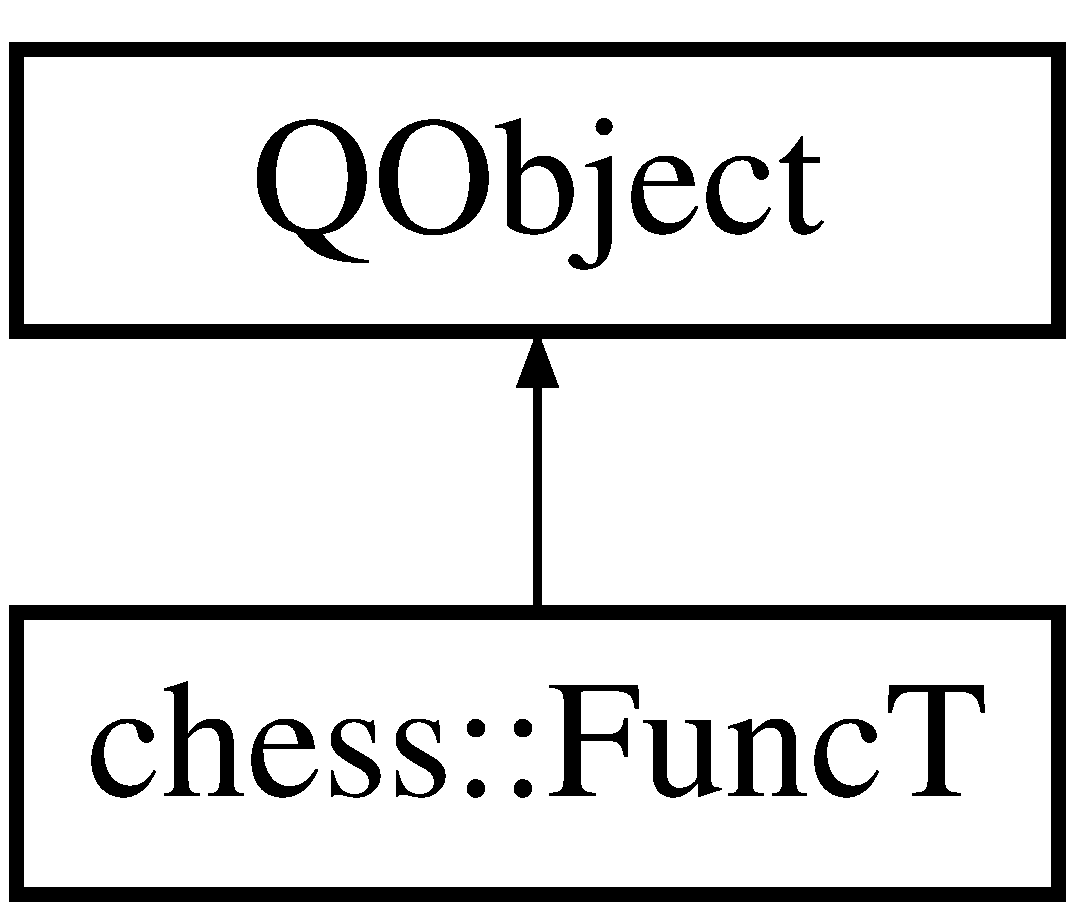
\includegraphics[height=2.000000cm]{classchess_1_1FuncT}
\end{center}
\end{figure}
\subsection*{Public Slots}
\begin{DoxyCompactItemize}
\item 
\hypertarget{classchess_1_1FuncT_a88ae07450073354a6fe3561020f5990a}{void {\bfseries print\-Info} (Q\-String info)}\label{classchess_1_1FuncT_a88ae07450073354a6fe3561020f5990a}

\item 
\hypertarget{classchess_1_1FuncT_a519de891915d878ff5ddd0aacbe46571}{void {\bfseries print\-Bestmove} (const Q\-String \&move)}\label{classchess_1_1FuncT_a519de891915d878ff5ddd0aacbe46571}

\end{DoxyCompactItemize}
\subsection*{Public Member Functions}
\begin{DoxyCompactItemize}
\item 
\hypertarget{classchess_1_1FuncT_a46095d8ecf17a52d350f20a8c0870304}{{\bfseries Func\-T} (Q\-Object $\ast$parent=0)}\label{classchess_1_1FuncT_a46095d8ecf17a52d350f20a8c0870304}

\item 
\hypertarget{classchess_1_1FuncT_a692a5fac8edc90ec114ceff4c1a3671d}{void {\bfseries run\-\_\-pgnt} ()}\label{classchess_1_1FuncT_a692a5fac8edc90ec114ceff4c1a3671d}

\item 
\hypertarget{classchess_1_1FuncT_a4b403881f0ac946209b25946e2fcb530}{void {\bfseries run\-\_\-sant} ()}\label{classchess_1_1FuncT_a4b403881f0ac946209b25946e2fcb530}

\item 
\hypertarget{classchess_1_1FuncT_aeee31af9d7148fc54f799d2a79846c8f}{void {\bfseries run\-\_\-pertf} ()}\label{classchess_1_1FuncT_aeee31af9d7148fc54f799d2a79846c8f}

\item 
\hypertarget{classchess_1_1FuncT_aa2aa0cceb2dee0ec37c67fac47b2d79c}{void {\bfseries run\-\_\-pgn\-\_\-scant} ()}\label{classchess_1_1FuncT_aa2aa0cceb2dee0ec37c67fac47b2d79c}

\item 
\hypertarget{classchess_1_1FuncT_aa56f686abbb5b84c1c34ecbe7bf0cbda}{void {\bfseries run\-\_\-ucit} ()}\label{classchess_1_1FuncT_aa56f686abbb5b84c1c34ecbe7bf0cbda}

\end{DoxyCompactItemize}


The documentation for this class was generated from the following files\-:\begin{DoxyCompactItemize}
\item 
funct.\-h\item 
funct.\-cpp\end{DoxyCompactItemize}

\hypertarget{classchess_1_1Game}{\section{chess\-:\-:Game Class Reference}
\label{classchess_1_1Game}\index{chess\-::\-Game@{chess\-::\-Game}}
}
\subsection*{Public Member Functions}
\begin{DoxyCompactItemize}
\item 
\hypertarget{classchess_1_1Game_adca9940d7473dcac562c2934d0e762a9}{\hyperlink{classchess_1_1Game_adca9940d7473dcac562c2934d0e762a9}{Game} ()}\label{classchess_1_1Game_adca9940d7473dcac562c2934d0e762a9}

\begin{DoxyCompactList}\small\item\em \hyperlink{classchess_1_1Game}{Game} essentially a tree of \hyperlink{classchess_1_1GameNode}{Game\-Node} objects that represents a game. Default root node has a board position which is empty. \end{DoxyCompactList}\item 
\hyperlink{classchess_1_1GameNode}{Game\-Node} $\ast$ \hyperlink{classchess_1_1Game_ac8425c271f2d8365f813e5e169f7d1ed}{get\-Root\-Node} ()
\begin{DoxyCompactList}\small\item\em get\-Root\-Node returns the root node of the game \end{DoxyCompactList}\item 
\hyperlink{classchess_1_1GameNode}{Game\-Node} $\ast$ \hyperlink{classchess_1_1Game_a77233d7bfe997d113300b3c4333258d4}{get\-Current\-Node} ()
\begin{DoxyCompactList}\small\item\em get\-Current\-Node returns the current node. The current node is a pointer to a node in the tree and used e.\-g. for the node of the last move \end{DoxyCompactList}\item 
int \hyperlink{classchess_1_1Game_aae095f72d044192f348c1f0b740aae32}{get\-Result} ()
\begin{DoxyCompactList}\small\item\em get\-Result returns the result of the game \end{DoxyCompactList}\item 
void \hyperlink{classchess_1_1Game_a9b10980b3b16b19c73e07034840ea3ea}{set\-Result} (int r)
\begin{DoxyCompactList}\small\item\em set\-Result sets the result of the game \end{DoxyCompactList}\item 
void \hyperlink{classchess_1_1Game_a5a5346e8f2b6d5063c2e1c8f892a08ed}{apply\-Move} (\hyperlink{classchess_1_1Move}{Move} $\ast$m)
\begin{DoxyCompactList}\small\item\em apply\-Move apply a move to the current node, and change the node to the resulting new node (or existing node) if a child node for this move already exists. There is no check if the supplied move is legal! \end{DoxyCompactList}\item 
\hyperlink{classchess_1_1GameNode}{Game\-Node} $\ast$ \hyperlink{classchess_1_1Game_ac018e45f806510247404ba56feda568c}{find\-Node\-By\-Id} (int id)
\begin{DoxyCompactList}\small\item\em find\-Node\-By\-Id each \hyperlink{classchess_1_1GameNode}{Game\-Node} has a unique id (see class definition) this searches for and find the node given the supplied id throw std\-::invalid\-\_\-argument if there exists no node with the id \end{DoxyCompactList}\item 
void \hyperlink{classchess_1_1Game_a07156dfe4b3dff8991350dcb38c9508e}{set\-Current} (\hyperlink{classchess_1_1GameNode}{Game\-Node} $\ast$new\-\_\-current)
\begin{DoxyCompactList}\small\item\em set\-Current set the current pointer to the supplied node. There is no validity check whether the node is actually a node in the game tree. \end{DoxyCompactList}\item 
void \hyperlink{classchess_1_1Game_af508607bc605b8974c2a393f0b3ecae1}{set\-Root} (\hyperlink{classchess_1_1GameNode}{Game\-Node} $\ast$new\-\_\-root)
\begin{DoxyCompactList}\small\item\em set\-Root sets the root node pointer to the supplied node. Really just that. Beware of memory leaks when using this function, as nodes below the old root might become inaccessible \end{DoxyCompactList}\item 
\hypertarget{classchess_1_1Game_a254acf6e5423d9f9332f6f43f0455cb7}{void \hyperlink{classchess_1_1Game_a254acf6e5423d9f9332f6f43f0455cb7}{go\-To\-Main\-Line\-Child} ()}\label{classchess_1_1Game_a254acf6e5423d9f9332f6f43f0455cb7}

\begin{DoxyCompactList}\small\item\em go\-To\-Main\-Line\-Child moves the current node pointer one down to the mainline (zeroth) variation (if it exists), otherwise keeps the pointer at the current node \end{DoxyCompactList}\item 
void \hyperlink{classchess_1_1Game_a6b634132c4549290bd1bedd2444f7072}{go\-To\-Child} (int idx\-\_\-child)
\begin{DoxyCompactList}\small\item\em go\-To\-Child moves the current node poiner to the child at index idx\-\_\-child. If the index is out of range, keeps the pointer at the current node. \end{DoxyCompactList}\item 
\hypertarget{classchess_1_1Game_a192a5708f9cc181ceff6bfd0eb2fc883}{void \hyperlink{classchess_1_1Game_a192a5708f9cc181ceff6bfd0eb2fc883}{go\-To\-Parent} ()}\label{classchess_1_1Game_a192a5708f9cc181ceff6bfd0eb2fc883}

\begin{DoxyCompactList}\small\item\em go\-To\-Parent moves current node pointer to the parent node (if exists). keeps pointer at existing node if already at root \end{DoxyCompactList}\item 
\hypertarget{classchess_1_1Game_aa14b8365fc4c0a472b00a214fd67e302}{void \hyperlink{classchess_1_1Game_aa14b8365fc4c0a472b00a214fd67e302}{go\-To\-Root} ()}\label{classchess_1_1Game_aa14b8365fc4c0a472b00a214fd67e302}

\begin{DoxyCompactList}\small\item\em go\-To\-Root moves current pointer to the root node of the game \end{DoxyCompactList}\item 
\hypertarget{classchess_1_1Game_ad421efa010dedf785ad2c6211910167f}{void \hyperlink{classchess_1_1Game_ad421efa010dedf785ad2c6211910167f}{go\-To\-End} ()}\label{classchess_1_1Game_ad421efa010dedf785ad2c6211910167f}

\begin{DoxyCompactList}\small\item\em go\-To\-End starting at the current node, moves the current node pointer down among all mainline until reaching a leaf \end{DoxyCompactList}\item 
void \hyperlink{classchess_1_1Game_a5232c5b68052202aa8167df619837912}{move\-Up} (\hyperlink{classchess_1_1GameNode}{Game\-Node} $\ast$node)
\begin{DoxyCompactList}\small\item\em move\-Up Suppose the supplied node is a child referenced at parent with index i, and there is another child of the parent with index i-\/1. Then this function switches these indexes. In other word, moves the supplied node variation one up. Has no effect, if node is root (i.\-e. has no parent) or is already the mainline (i.\-e. the zeroth) child of parent. \end{DoxyCompactList}\item 
void \hyperlink{classchess_1_1Game_a0c87b025f3d1aceaded403d62c40f567}{move\-Down} (\hyperlink{classchess_1_1GameNode}{Game\-Node} $\ast$node)
\begin{DoxyCompactList}\small\item\em move\-Down Reverse of \hyperlink{classchess_1_1Game_a5232c5b68052202aa8167df619837912}{move\-Up()}. \end{DoxyCompactList}\item 
void \hyperlink{classchess_1_1Game_aaca844dd847f3e163e9da9e990f30931}{del\-Variant} (\hyperlink{classchess_1_1GameNode}{Game\-Node} $\ast$node)
\begin{DoxyCompactList}\small\item\em del\-Variant deletes the whole variation on which the supplied node exists. I.\-e. moves up the tree to the root of the variation, and deletes everything below. sets current node pointer to the root of the variation. \end{DoxyCompactList}\item 
void \hyperlink{classchess_1_1Game_afb049584b03af5ce0d58f5feb6806a1f}{del\-Below} (\hyperlink{classchess_1_1GameNode}{Game\-Node} $\ast$node)
\begin{DoxyCompactList}\small\item\em del\-Below delete the subtree below the supplied node. Afterwards sets current node pointer to the supplied node. \end{DoxyCompactList}\item 
void \hyperlink{classchess_1_1Game_acb9da8af7684660ec3880f15143e051b}{remove\-Comment\-Rec} (\hyperlink{classchess_1_1GameNode}{Game\-Node} $\ast$node)
\begin{DoxyCompactList}\small\item\em remove\-Comment\-Rec removes comment at supplied node and recursively removes at all comments at nodes below the supplied node. \end{DoxyCompactList}\item 
\hypertarget{classchess_1_1Game_a37f62be6e55d2e3415f5e08016e9c038}{void \hyperlink{classchess_1_1Game_a37f62be6e55d2e3415f5e08016e9c038}{go\-To\-Leaf} ()}\label{classchess_1_1Game_a37f62be6e55d2e3415f5e08016e9c038}

\begin{DoxyCompactList}\small\item\em go\-To\-Leaf from the current node pointer, go down the mainlines until there are no more childs. \end{DoxyCompactList}\item 
void \hyperlink{classchess_1_1Game_ae7d450a354b5943cca2a60380f5152b4}{reset\-With\-New\-Root\-Board} (\hyperlink{classchess_1_1Board}{chess\-::\-Board} $\ast$new\-\_\-root\-\_\-board)
\begin{DoxyCompactList}\small\item\em reset\-With\-New\-Root\-Board delete the whole game tree, and set a new root node constructed with the supplied move. Essentially call this, if a new game has been requrested by the user, especially if the user has set up a custom board position. The supplied board M\-U\-S\-T be a valid board position. \end{DoxyCompactList}\item 
\hypertarget{classchess_1_1Game_a18ab6e0fd6ee734a9810886f57e87b5a}{void \hyperlink{classchess_1_1Game_a18ab6e0fd6ee734a9810886f57e87b5a}{remove\-All\-Comments} ()}\label{classchess_1_1Game_a18ab6e0fd6ee734a9810886f57e87b5a}

\begin{DoxyCompactList}\small\item\em remove\-All\-Comments iterates through the tree, and removes every comment from each \hyperlink{classchess_1_1GameNode}{Game\-Node} \end{DoxyCompactList}\item 
\hypertarget{classchess_1_1Game_a0bad886ab7d0041ae777afa84667dca3}{void \hyperlink{classchess_1_1Game_a0bad886ab7d0041ae777afa84667dca3}{remove\-All\-Variants} ()}\label{classchess_1_1Game_a0bad886ab7d0041ae777afa84667dca3}

\begin{DoxyCompactList}\small\item\em remove\-All\-Variants iterates through the tree and keeps only the mainlines (i.\-e. zeroth) variations if there are more than one child in a \hyperlink{classchess_1_1GameNode}{Game\-Node} \end{DoxyCompactList}\item 
\hypertarget{classchess_1_1Game_afa39fec09e0c6aa13b0c03e7ce1dbc44}{void \hyperlink{classchess_1_1Game_afa39fec09e0c6aa13b0c03e7ce1dbc44}{clear\-Headers} ()}\label{classchess_1_1Game_afa39fec09e0c6aa13b0c03e7ce1dbc44}

\begin{DoxyCompactList}\small\item\em clear\-Headers deletes all headers entries. \end{DoxyCompactList}\end{DoxyCompactItemize}
\subsection*{Public Attributes}
\begin{DoxyCompactItemize}
\item 
\hypertarget{classchess_1_1Game_a80169885e34540646a724431673067e5}{bool \hyperlink{classchess_1_1Game_a80169885e34540646a724431673067e5}{tree\-Was\-Changed}}\label{classchess_1_1Game_a80169885e34540646a724431673067e5}

\begin{DoxyCompactList}\small\item\em tree\-Was\-Changed this variable is set to true (either by a member function of \hyperlink{classchess_1_1Game}{Game} or manually) if an operation was carried out that changed fundamentally the tree structure In other words, if the this variable is true, an existing G\-U\-I representation of the \hyperlink{classchess_1_1Game}{Game} tree must be likely be reconstructed \end{DoxyCompactList}\item 
\hypertarget{classchess_1_1Game_a6c48e9e2ec4e304baf425dc9ab493b17}{Q\-Map$<$ Q\-String, Q\-String $>$ $\ast$ \hyperlink{classchess_1_1Game_a6c48e9e2ec4e304baf425dc9ab493b17}{headers}}\label{classchess_1_1Game_a6c48e9e2ec4e304baf425dc9ab493b17}

\begin{DoxyCompactList}\small\item\em headers contains the game headers. During construction of a \hyperlink{classchess_1_1Game}{Game} object there will always be the 7tag roster index entries (albeit initialized to empty field) \end{DoxyCompactList}\end{DoxyCompactItemize}


\subsection{Member Function Documentation}
\hypertarget{classchess_1_1Game_a5a5346e8f2b6d5063c2e1c8f892a08ed}{\index{chess\-::\-Game@{chess\-::\-Game}!apply\-Move@{apply\-Move}}
\index{apply\-Move@{apply\-Move}!chess::Game@{chess\-::\-Game}}
\subsubsection[{apply\-Move}]{\setlength{\rightskip}{0pt plus 5cm}void chess\-::\-Game\-::apply\-Move (
\begin{DoxyParamCaption}
\item[{{\bf Move} $\ast$}]{m}
\end{DoxyParamCaption}
)}}\label{classchess_1_1Game_a5a5346e8f2b6d5063c2e1c8f892a08ed}


apply\-Move apply a move to the current node, and change the node to the resulting new node (or existing node) if a child node for this move already exists. There is no check if the supplied move is legal! 


\begin{DoxyParams}{Parameters}
{\em m} & the move to apply on the current board. \\
\hline
\end{DoxyParams}
\hypertarget{classchess_1_1Game_afb049584b03af5ce0d58f5feb6806a1f}{\index{chess\-::\-Game@{chess\-::\-Game}!del\-Below@{del\-Below}}
\index{del\-Below@{del\-Below}!chess::Game@{chess\-::\-Game}}
\subsubsection[{del\-Below}]{\setlength{\rightskip}{0pt plus 5cm}void chess\-::\-Game\-::del\-Below (
\begin{DoxyParamCaption}
\item[{{\bf Game\-Node} $\ast$}]{node}
\end{DoxyParamCaption}
)}}\label{classchess_1_1Game_afb049584b03af5ce0d58f5feb6806a1f}


del\-Below delete the subtree below the supplied node. Afterwards sets current node pointer to the supplied node. 


\begin{DoxyParams}{Parameters}
{\em node} & \\
\hline
\end{DoxyParams}
\hypertarget{classchess_1_1Game_aaca844dd847f3e163e9da9e990f30931}{\index{chess\-::\-Game@{chess\-::\-Game}!del\-Variant@{del\-Variant}}
\index{del\-Variant@{del\-Variant}!chess::Game@{chess\-::\-Game}}
\subsubsection[{del\-Variant}]{\setlength{\rightskip}{0pt plus 5cm}void chess\-::\-Game\-::del\-Variant (
\begin{DoxyParamCaption}
\item[{{\bf Game\-Node} $\ast$}]{node}
\end{DoxyParamCaption}
)}}\label{classchess_1_1Game_aaca844dd847f3e163e9da9e990f30931}


del\-Variant deletes the whole variation on which the supplied node exists. I.\-e. moves up the tree to the root of the variation, and deletes everything below. sets current node pointer to the root of the variation. 


\begin{DoxyParams}{Parameters}
{\em node} & \\
\hline
\end{DoxyParams}
\hypertarget{classchess_1_1Game_ac018e45f806510247404ba56feda568c}{\index{chess\-::\-Game@{chess\-::\-Game}!find\-Node\-By\-Id@{find\-Node\-By\-Id}}
\index{find\-Node\-By\-Id@{find\-Node\-By\-Id}!chess::Game@{chess\-::\-Game}}
\subsubsection[{find\-Node\-By\-Id}]{\setlength{\rightskip}{0pt plus 5cm}{\bf Game\-Node} $\ast$ chess\-::\-Game\-::find\-Node\-By\-Id (
\begin{DoxyParamCaption}
\item[{int}]{id}
\end{DoxyParamCaption}
)}}\label{classchess_1_1Game_ac018e45f806510247404ba56feda568c}


find\-Node\-By\-Id each \hyperlink{classchess_1_1GameNode}{Game\-Node} has a unique id (see class definition) this searches for and find the node given the supplied id throw std\-::invalid\-\_\-argument if there exists no node with the id 


\begin{DoxyParams}{Parameters}
{\em id} & the node id \\
\hline
\end{DoxyParams}
\begin{DoxyReturn}{Returns}
gamenode with the supplied id 
\end{DoxyReturn}
\hypertarget{classchess_1_1Game_a77233d7bfe997d113300b3c4333258d4}{\index{chess\-::\-Game@{chess\-::\-Game}!get\-Current\-Node@{get\-Current\-Node}}
\index{get\-Current\-Node@{get\-Current\-Node}!chess::Game@{chess\-::\-Game}}
\subsubsection[{get\-Current\-Node}]{\setlength{\rightskip}{0pt plus 5cm}{\bf Game\-Node} $\ast$ chess\-::\-Game\-::get\-Current\-Node (
\begin{DoxyParamCaption}
{}
\end{DoxyParamCaption}
)}}\label{classchess_1_1Game_a77233d7bfe997d113300b3c4333258d4}


get\-Current\-Node returns the current node. The current node is a pointer to a node in the tree and used e.\-g. for the node of the last move 

\begin{DoxyReturn}{Returns}

\end{DoxyReturn}
\hypertarget{classchess_1_1Game_aae095f72d044192f348c1f0b740aae32}{\index{chess\-::\-Game@{chess\-::\-Game}!get\-Result@{get\-Result}}
\index{get\-Result@{get\-Result}!chess::Game@{chess\-::\-Game}}
\subsubsection[{get\-Result}]{\setlength{\rightskip}{0pt plus 5cm}int chess\-::\-Game\-::get\-Result (
\begin{DoxyParamCaption}
{}
\end{DoxyParamCaption}
)}}\label{classchess_1_1Game_aae095f72d044192f348c1f0b740aae32}


get\-Result returns the result of the game 

\begin{DoxyReturn}{Returns}
R\-E\-S\-\_\-\-B\-L\-A\-C\-K\-\_\-\-W\-I\-N\-S or R\-E\-S\-\_\-\-D\-R\-A\-W or R\-E\-S\-\_\-\-W\-H\-I\-T\-E\-\_\-\-W\-I\-N\-S or R\-E\-S\-\_\-\-U\-N\-D\-E\-F 
\end{DoxyReturn}
\hypertarget{classchess_1_1Game_ac8425c271f2d8365f813e5e169f7d1ed}{\index{chess\-::\-Game@{chess\-::\-Game}!get\-Root\-Node@{get\-Root\-Node}}
\index{get\-Root\-Node@{get\-Root\-Node}!chess::Game@{chess\-::\-Game}}
\subsubsection[{get\-Root\-Node}]{\setlength{\rightskip}{0pt plus 5cm}{\bf Game\-Node} $\ast$ chess\-::\-Game\-::get\-Root\-Node (
\begin{DoxyParamCaption}
{}
\end{DoxyParamCaption}
)}}\label{classchess_1_1Game_ac8425c271f2d8365f813e5e169f7d1ed}


get\-Root\-Node returns the root node of the game 

\begin{DoxyReturn}{Returns}

\end{DoxyReturn}
\hypertarget{classchess_1_1Game_a6b634132c4549290bd1bedd2444f7072}{\index{chess\-::\-Game@{chess\-::\-Game}!go\-To\-Child@{go\-To\-Child}}
\index{go\-To\-Child@{go\-To\-Child}!chess::Game@{chess\-::\-Game}}
\subsubsection[{go\-To\-Child}]{\setlength{\rightskip}{0pt plus 5cm}void chess\-::\-Game\-::go\-To\-Child (
\begin{DoxyParamCaption}
\item[{int}]{idx\-\_\-child}
\end{DoxyParamCaption}
)}}\label{classchess_1_1Game_a6b634132c4549290bd1bedd2444f7072}


go\-To\-Child moves the current node poiner to the child at index idx\-\_\-child. If the index is out of range, keeps the pointer at the current node. 


\begin{DoxyParams}{Parameters}
{\em idx\-\_\-child} & the index of the variation of the child node \\
\hline
\end{DoxyParams}
\hypertarget{classchess_1_1Game_a0c87b025f3d1aceaded403d62c40f567}{\index{chess\-::\-Game@{chess\-::\-Game}!move\-Down@{move\-Down}}
\index{move\-Down@{move\-Down}!chess::Game@{chess\-::\-Game}}
\subsubsection[{move\-Down}]{\setlength{\rightskip}{0pt plus 5cm}void chess\-::\-Game\-::move\-Down (
\begin{DoxyParamCaption}
\item[{{\bf Game\-Node} $\ast$}]{node}
\end{DoxyParamCaption}
)}}\label{classchess_1_1Game_a0c87b025f3d1aceaded403d62c40f567}


move\-Down Reverse of \hyperlink{classchess_1_1Game_a5232c5b68052202aa8167df619837912}{move\-Up()}. 


\begin{DoxyParams}{Parameters}
{\em node} & \\
\hline
\end{DoxyParams}
\hypertarget{classchess_1_1Game_a5232c5b68052202aa8167df619837912}{\index{chess\-::\-Game@{chess\-::\-Game}!move\-Up@{move\-Up}}
\index{move\-Up@{move\-Up}!chess::Game@{chess\-::\-Game}}
\subsubsection[{move\-Up}]{\setlength{\rightskip}{0pt plus 5cm}void chess\-::\-Game\-::move\-Up (
\begin{DoxyParamCaption}
\item[{{\bf Game\-Node} $\ast$}]{node}
\end{DoxyParamCaption}
)}}\label{classchess_1_1Game_a5232c5b68052202aa8167df619837912}


move\-Up Suppose the supplied node is a child referenced at parent with index i, and there is another child of the parent with index i-\/1. Then this function switches these indexes. In other word, moves the supplied node variation one up. Has no effect, if node is root (i.\-e. has no parent) or is already the mainline (i.\-e. the zeroth) child of parent. 


\begin{DoxyParams}{Parameters}
{\em node} & The node that should be moved up \\
\hline
\end{DoxyParams}
\hypertarget{classchess_1_1Game_acb9da8af7684660ec3880f15143e051b}{\index{chess\-::\-Game@{chess\-::\-Game}!remove\-Comment\-Rec@{remove\-Comment\-Rec}}
\index{remove\-Comment\-Rec@{remove\-Comment\-Rec}!chess::Game@{chess\-::\-Game}}
\subsubsection[{remove\-Comment\-Rec}]{\setlength{\rightskip}{0pt plus 5cm}void chess\-::\-Game\-::remove\-Comment\-Rec (
\begin{DoxyParamCaption}
\item[{{\bf Game\-Node} $\ast$}]{node}
\end{DoxyParamCaption}
)}}\label{classchess_1_1Game_acb9da8af7684660ec3880f15143e051b}


remove\-Comment\-Rec removes comment at supplied node and recursively removes at all comments at nodes below the supplied node. 


\begin{DoxyParams}{Parameters}
{\em node} & the node to start with. \\
\hline
\end{DoxyParams}
\hypertarget{classchess_1_1Game_ae7d450a354b5943cca2a60380f5152b4}{\index{chess\-::\-Game@{chess\-::\-Game}!reset\-With\-New\-Root\-Board@{reset\-With\-New\-Root\-Board}}
\index{reset\-With\-New\-Root\-Board@{reset\-With\-New\-Root\-Board}!chess::Game@{chess\-::\-Game}}
\subsubsection[{reset\-With\-New\-Root\-Board}]{\setlength{\rightskip}{0pt plus 5cm}void chess\-::\-Game\-::reset\-With\-New\-Root\-Board (
\begin{DoxyParamCaption}
\item[{{\bf chess\-::\-Board} $\ast$}]{new\-\_\-root\-\_\-board}
\end{DoxyParamCaption}
)}}\label{classchess_1_1Game_ae7d450a354b5943cca2a60380f5152b4}


reset\-With\-New\-Root\-Board delete the whole game tree, and set a new root node constructed with the supplied move. Essentially call this, if a new game has been requrested by the user, especially if the user has set up a custom board position. The supplied board M\-U\-S\-T be a valid board position. 


\begin{DoxyParams}{Parameters}
{\em new\-\_\-root\-\_\-board} & The chess board to construct the root node. \\
\hline
\end{DoxyParams}
\hypertarget{classchess_1_1Game_a07156dfe4b3dff8991350dcb38c9508e}{\index{chess\-::\-Game@{chess\-::\-Game}!set\-Current@{set\-Current}}
\index{set\-Current@{set\-Current}!chess::Game@{chess\-::\-Game}}
\subsubsection[{set\-Current}]{\setlength{\rightskip}{0pt plus 5cm}void chess\-::\-Game\-::set\-Current (
\begin{DoxyParamCaption}
\item[{{\bf Game\-Node} $\ast$}]{new\-\_\-current}
\end{DoxyParamCaption}
)}}\label{classchess_1_1Game_a07156dfe4b3dff8991350dcb38c9508e}


set\-Current set the current pointer to the supplied node. There is no validity check whether the node is actually a node in the game tree. 


\begin{DoxyParams}{Parameters}
{\em new\-\_\-current} & pointer to the node \\
\hline
\end{DoxyParams}
\hypertarget{classchess_1_1Game_a9b10980b3b16b19c73e07034840ea3ea}{\index{chess\-::\-Game@{chess\-::\-Game}!set\-Result@{set\-Result}}
\index{set\-Result@{set\-Result}!chess::Game@{chess\-::\-Game}}
\subsubsection[{set\-Result}]{\setlength{\rightskip}{0pt plus 5cm}void chess\-::\-Game\-::set\-Result (
\begin{DoxyParamCaption}
\item[{int}]{r}
\end{DoxyParamCaption}
)}}\label{classchess_1_1Game_a9b10980b3b16b19c73e07034840ea3ea}


set\-Result sets the result of the game 


\begin{DoxyParams}{Parameters}
{\em r} & see \hyperlink{classchess_1_1Game_aae095f72d044192f348c1f0b740aae32}{get\-Result()} \\
\hline
\end{DoxyParams}
\hypertarget{classchess_1_1Game_af508607bc605b8974c2a393f0b3ecae1}{\index{chess\-::\-Game@{chess\-::\-Game}!set\-Root@{set\-Root}}
\index{set\-Root@{set\-Root}!chess::Game@{chess\-::\-Game}}
\subsubsection[{set\-Root}]{\setlength{\rightskip}{0pt plus 5cm}void chess\-::\-Game\-::set\-Root (
\begin{DoxyParamCaption}
\item[{{\bf Game\-Node} $\ast$}]{new\-\_\-root}
\end{DoxyParamCaption}
)}}\label{classchess_1_1Game_af508607bc605b8974c2a393f0b3ecae1}


set\-Root sets the root node pointer to the supplied node. Really just that. Beware of memory leaks when using this function, as nodes below the old root might become inaccessible 


\begin{DoxyParams}{Parameters}
{\em new\-\_\-root} & \\
\hline
\end{DoxyParams}


The documentation for this class was generated from the following files\-:\begin{DoxyCompactItemize}
\item 
chess/game.\-h\item 
chess/game.\-cpp\end{DoxyCompactItemize}

\hypertarget{classchess_1_1GameNode}{\section{chess\-:\-:Game\-Node Class Reference}
\label{classchess_1_1GameNode}\index{chess\-::\-Game\-Node@{chess\-::\-Game\-Node}}
}
\subsection*{Public Member Functions}
\begin{DoxyCompactItemize}
\item 
\hypertarget{classchess_1_1GameNode_ae0efe18314ec18e2a5cd2c1e5c3bd741}{\hyperlink{classchess_1_1GameNode_ae0efe18314ec18e2a5cd2c1e5c3bd741}{$\sim$\-Game\-Node} ()}\label{classchess_1_1GameNode_ae0efe18314ec18e2a5cd2c1e5c3bd741}

\begin{DoxyCompactList}\small\item\em The destructor does N\-O\-T delete child nodes. You are responsible yourself for deleting child nodes. In general, member functions from Game() to manage the tree should be used. \end{DoxyCompactList}\item 
int \hyperlink{classchess_1_1GameNode_a8ca2222d9ea74fa3c3e581b90b446f20}{get\-Id} ()
\begin{DoxyCompactList}\small\item\em get\-Id each game node is assigned a unique id automatically during construction. \end{DoxyCompactList}\item 
\hyperlink{classchess_1_1Board}{Board} $\ast$ \hyperlink{classchess_1_1GameNode_a68758d5555d7e01f13dd7e5685fa7fdc}{get\-Board} ()
\begin{DoxyCompactList}\small\item\em get\-Board \end{DoxyCompactList}\item 
void \hyperlink{classchess_1_1GameNode_a285593d02086c1c6bb30c852b0b41d5f}{set\-Board} (\hyperlink{classchess_1_1Board}{Board} $\ast$b)
\begin{DoxyCompactList}\small\item\em set\-Board deletes the old board of this node, and sets the supplied board as the new one. Does no validity checks of the board position \end{DoxyCompactList}\item 
Q\-String \hyperlink{classchess_1_1GameNode_aa56312861ca85710a7979b66427fd1cd}{get\-San} ()
\begin{DoxyCompactList}\small\item\em get\-San returns san string of move that lead to this node. \end{DoxyCompactList}\item 
\hyperlink{classchess_1_1GameNode}{Game\-Node} $\ast$ \hyperlink{classchess_1_1GameNode_a3893ddd950c675600e030d8e3817e48a}{root} ()
\begin{DoxyCompactList}\small\item\em root returns root node of the game \end{DoxyCompactList}\item 
\hyperlink{classchess_1_1GameNode}{Game\-Node} $\ast$ \hyperlink{classchess_1_1GameNode_ac35bd1ef7f0ba9ce43306d224d9b6839}{get\-Parent} ()
\begin{DoxyCompactList}\small\item\em get\-Parent returns the parent of the node. null if there is no parent (e.\-g. root node or freshly created) \end{DoxyCompactList}\item 
\hyperlink{classchess_1_1Move}{Move} $\ast$ \hyperlink{classchess_1_1GameNode_a7ca0e6953eef522ac8dbfd5869ed99a8}{get\-Move} ()
\begin{DoxyCompactList}\small\item\em get\-Move returns move leading to this node. Null if there is no move (e.\-g. root node) \end{DoxyCompactList}\item 
void \hyperlink{classchess_1_1GameNode_a7c501e59559bf59aac7cb5337151e6c5}{set\-Move} (\hyperlink{classchess_1_1Move}{Move} $\ast$m)
\begin{DoxyCompactList}\small\item\em set\-Move set the move that leads to this game node to m. There is no validity or consistency check. \end{DoxyCompactList}\item 
void \hyperlink{classchess_1_1GameNode_a8a3dcdb5d5dedc45e1cbf78405f137e7}{set\-Parent} (\hyperlink{classchess_1_1GameNode}{Game\-Node} $\ast$g)
\begin{DoxyCompactList}\small\item\em set\-Parent Set the parent to the supplied \hyperlink{classchess_1_1Game}{Game} Node. No validity / consistency checks. Old parent is not deleted. \end{DoxyCompactList}\item 
void \hyperlink{classchess_1_1GameNode_a706311ef7dfc985b5bb9afc1802371e2}{set\-Comment} (Q\-String \&c)
\begin{DoxyCompactList}\small\item\em set\-Comment Set comment for this node to supplied textstring. \end{DoxyCompactList}\item 
Q\-String \hyperlink{classchess_1_1GameNode_af9256a164fa665dda2b6310af1d3a7d3}{get\-Comment} ()
\begin{DoxyCompactList}\small\item\em get\-Comment returns the comment for this node. Empty text string if there is no comment. \end{DoxyCompactList}\item 
\hyperlink{classchess_1_1GameNode}{Game\-Node} $\ast$ \hyperlink{classchess_1_1GameNode_a181e93f7fdb90e82f259f4add006f389}{get\-Variation} (int i)
\begin{DoxyCompactList}\small\item\em get\-Variation get the variation (i.\-e. the child) at index i \end{DoxyCompactList}\item 
Q\-List$<$ \hyperlink{classchess_1_1GameNode}{Game\-Node} $\ast$ $>$ $\ast$ \hyperlink{classchess_1_1GameNode_a901705a202fb5d5b7795e9c49e1f003c}{get\-Variations} ()
\begin{DoxyCompactList}\small\item\em get\-Variations returns list of all child nodes, i.\-e. all variations starting in this position. \end{DoxyCompactList}\item 
void \hyperlink{classchess_1_1GameNode_a79a49a66ec0ad97dfa1f86af3135c1b4}{add\-Variation} (\hyperlink{classchess_1_1GameNode}{Game\-Node} $\ast$g)
\begin{DoxyCompactList}\small\item\em add\-Variation adds a new variation by putting the supplied game node at the end of the list of all variations. sets parent of g to this node. Does N\-O\-T check whether the variation already exists. \end{DoxyCompactList}\item 
bool \hyperlink{classchess_1_1GameNode_a53453fb45ecf163d4b7c09d7f7d7166d}{has\-Variations} ()
\begin{DoxyCompactList}\small\item\em has\-Variations checks whether the node as variations, i.\-e. more than one (mainline) variations \end{DoxyCompactList}\item 
bool \hyperlink{classchess_1_1GameNode_a727d2e54a5c38bb082e356f254e15400}{is\-Leaf} ()
\begin{DoxyCompactList}\small\item\em is\-Leaf checks whether node is leaf. \end{DoxyCompactList}\item 
void \hyperlink{classchess_1_1GameNode_aa2e6bfdf0cedd649fd643b8d27be885a}{add\-Nag} (int n)
\begin{DoxyCompactList}\small\item\em add\-Nag add numeric annotation glyph (see P\-G\-N standard) \end{DoxyCompactList}\item 
Q\-List$<$ int $>$ $\ast$ \hyperlink{classchess_1_1GameNode_a7a96e223a5f25429e001646d51404704}{get\-Nags} ()
\begin{DoxyCompactList}\small\item\em get\-Nags returns all numeric annotation glyphs (see P\-G\-N standard) \end{DoxyCompactList}\item 
Q\-List$<$ \hyperlink{structchess_1_1Arrow}{Arrow} $\ast$ $>$ $\ast$ \hyperlink{classchess_1_1GameNode_a4a5615b47f4f284d60b501e3f546f8da}{get\-Arrows} ()
\begin{DoxyCompactList}\small\item\em get\-Arrows returns a list with all arrows for this node. Arrows are just annotations done by the user for illustrations. \end{DoxyCompactList}\item 
Q\-List$<$ \hyperlink{structchess_1_1ColoredField}{Colored\-Field} $\ast$ $>$ $\ast$ \hyperlink{classchess_1_1GameNode_a4971268bae92d4341b59fc3b73b1031d}{get\-Colored\-Fields} ()
\begin{DoxyCompactList}\small\item\em get\-Colored\-Fields returns list of colored fields. Such fields are juts highlighted fields done by the user for illustration. \end{DoxyCompactList}\item 
void \hyperlink{classchess_1_1GameNode_ae339f67fc19405804df8c5ba8a63bd50}{add\-Or\-Del\-Arrow} (\hyperlink{structchess_1_1Arrow}{Arrow} $\ast$a)
\begin{DoxyCompactList}\small\item\em add\-Or\-Del\-Arrow adds (if the supplied arrow does not exist) or removes (if the node has that arrow already) and arrow from the board \end{DoxyCompactList}\item 
void \hyperlink{classchess_1_1GameNode_ae8846b9c88b9b59075e84e4346576f1d}{add\-Or\-Del\-Colored\-Field} (\hyperlink{structchess_1_1ColoredField}{Colored\-Field} $\ast$c)
\begin{DoxyCompactList}\small\item\em add\-Or\-Del\-Colored\-Field deletes color (field is already highlighted) or colorizes (field is plain) a board field. \end{DoxyCompactList}\end{DoxyCompactItemize}
\subsection*{Static Protected Member Functions}
\begin{DoxyCompactItemize}
\item 
\hypertarget{classchess_1_1GameNode_aa9d35a6c543e11213bdd0f49d5a3520e}{static int {\bfseries init\-Id} ()}\label{classchess_1_1GameNode_aa9d35a6c543e11213bdd0f49d5a3520e}

\end{DoxyCompactItemize}


\subsection{Member Function Documentation}
\hypertarget{classchess_1_1GameNode_aa2e6bfdf0cedd649fd643b8d27be885a}{\index{chess\-::\-Game\-Node@{chess\-::\-Game\-Node}!add\-Nag@{add\-Nag}}
\index{add\-Nag@{add\-Nag}!chess::GameNode@{chess\-::\-Game\-Node}}
\subsubsection[{add\-Nag}]{\setlength{\rightskip}{0pt plus 5cm}void chess\-::\-Game\-Node\-::add\-Nag (
\begin{DoxyParamCaption}
\item[{int}]{n}
\end{DoxyParamCaption}
)}}\label{classchess_1_1GameNode_aa2e6bfdf0cedd649fd643b8d27be885a}


add\-Nag add numeric annotation glyph (see P\-G\-N standard) 


\begin{DoxyParams}{Parameters}
{\em n} & N\-A\-G code \\
\hline
\end{DoxyParams}
\hypertarget{classchess_1_1GameNode_ae339f67fc19405804df8c5ba8a63bd50}{\index{chess\-::\-Game\-Node@{chess\-::\-Game\-Node}!add\-Or\-Del\-Arrow@{add\-Or\-Del\-Arrow}}
\index{add\-Or\-Del\-Arrow@{add\-Or\-Del\-Arrow}!chess::GameNode@{chess\-::\-Game\-Node}}
\subsubsection[{add\-Or\-Del\-Arrow}]{\setlength{\rightskip}{0pt plus 5cm}void chess\-::\-Game\-Node\-::add\-Or\-Del\-Arrow (
\begin{DoxyParamCaption}
\item[{{\bf Arrow} $\ast$}]{a}
\end{DoxyParamCaption}
)}}\label{classchess_1_1GameNode_ae339f67fc19405804df8c5ba8a63bd50}


add\-Or\-Del\-Arrow adds (if the supplied arrow does not exist) or removes (if the node has that arrow already) and arrow from the board 


\begin{DoxyParams}{Parameters}
{\em a} & the arrow that is supposed to be deleted or added \\
\hline
\end{DoxyParams}
\hypertarget{classchess_1_1GameNode_ae8846b9c88b9b59075e84e4346576f1d}{\index{chess\-::\-Game\-Node@{chess\-::\-Game\-Node}!add\-Or\-Del\-Colored\-Field@{add\-Or\-Del\-Colored\-Field}}
\index{add\-Or\-Del\-Colored\-Field@{add\-Or\-Del\-Colored\-Field}!chess::GameNode@{chess\-::\-Game\-Node}}
\subsubsection[{add\-Or\-Del\-Colored\-Field}]{\setlength{\rightskip}{0pt plus 5cm}void chess\-::\-Game\-Node\-::add\-Or\-Del\-Colored\-Field (
\begin{DoxyParamCaption}
\item[{{\bf Colored\-Field} $\ast$}]{c}
\end{DoxyParamCaption}
)}}\label{classchess_1_1GameNode_ae8846b9c88b9b59075e84e4346576f1d}


add\-Or\-Del\-Colored\-Field deletes color (field is already highlighted) or colorizes (field is plain) a board field. 


\begin{DoxyParams}{Parameters}
{\em c} & the colored field that is supposed to be deleted or added \\
\hline
\end{DoxyParams}
\hypertarget{classchess_1_1GameNode_a79a49a66ec0ad97dfa1f86af3135c1b4}{\index{chess\-::\-Game\-Node@{chess\-::\-Game\-Node}!add\-Variation@{add\-Variation}}
\index{add\-Variation@{add\-Variation}!chess::GameNode@{chess\-::\-Game\-Node}}
\subsubsection[{add\-Variation}]{\setlength{\rightskip}{0pt plus 5cm}void chess\-::\-Game\-Node\-::add\-Variation (
\begin{DoxyParamCaption}
\item[{{\bf Game\-Node} $\ast$}]{g}
\end{DoxyParamCaption}
)}}\label{classchess_1_1GameNode_a79a49a66ec0ad97dfa1f86af3135c1b4}


add\-Variation adds a new variation by putting the supplied game node at the end of the list of all variations. sets parent of g to this node. Does N\-O\-T check whether the variation already exists. 


\begin{DoxyParams}{Parameters}
{\em g} & the (new) child node. \\
\hline
\end{DoxyParams}
\hypertarget{classchess_1_1GameNode_a4a5615b47f4f284d60b501e3f546f8da}{\index{chess\-::\-Game\-Node@{chess\-::\-Game\-Node}!get\-Arrows@{get\-Arrows}}
\index{get\-Arrows@{get\-Arrows}!chess::GameNode@{chess\-::\-Game\-Node}}
\subsubsection[{get\-Arrows}]{\setlength{\rightskip}{0pt plus 5cm}Q\-List$<$ {\bf Arrow} $\ast$ $>$ $\ast$ chess\-::\-Game\-Node\-::get\-Arrows (
\begin{DoxyParamCaption}
{}
\end{DoxyParamCaption}
)}}\label{classchess_1_1GameNode_a4a5615b47f4f284d60b501e3f546f8da}


get\-Arrows returns a list with all arrows for this node. Arrows are just annotations done by the user for illustrations. 

\begin{DoxyReturn}{Returns}
list of arrows 
\end{DoxyReturn}
\hypertarget{classchess_1_1GameNode_a68758d5555d7e01f13dd7e5685fa7fdc}{\index{chess\-::\-Game\-Node@{chess\-::\-Game\-Node}!get\-Board@{get\-Board}}
\index{get\-Board@{get\-Board}!chess::GameNode@{chess\-::\-Game\-Node}}
\subsubsection[{get\-Board}]{\setlength{\rightskip}{0pt plus 5cm}{\bf Board} $\ast$ chess\-::\-Game\-Node\-::get\-Board (
\begin{DoxyParamCaption}
{}
\end{DoxyParamCaption}
)}}\label{classchess_1_1GameNode_a68758d5555d7e01f13dd7e5685fa7fdc}


get\-Board 

\begin{DoxyReturn}{Returns}
\hyperlink{classchess_1_1Board}{Board} of current node 
\end{DoxyReturn}
\hypertarget{classchess_1_1GameNode_a4971268bae92d4341b59fc3b73b1031d}{\index{chess\-::\-Game\-Node@{chess\-::\-Game\-Node}!get\-Colored\-Fields@{get\-Colored\-Fields}}
\index{get\-Colored\-Fields@{get\-Colored\-Fields}!chess::GameNode@{chess\-::\-Game\-Node}}
\subsubsection[{get\-Colored\-Fields}]{\setlength{\rightskip}{0pt plus 5cm}Q\-List$<$ {\bf Colored\-Field} $\ast$ $>$ $\ast$ chess\-::\-Game\-Node\-::get\-Colored\-Fields (
\begin{DoxyParamCaption}
{}
\end{DoxyParamCaption}
)}}\label{classchess_1_1GameNode_a4971268bae92d4341b59fc3b73b1031d}


get\-Colored\-Fields returns list of colored fields. Such fields are juts highlighted fields done by the user for illustration. 

\begin{DoxyReturn}{Returns}
list of color fields 
\end{DoxyReturn}
\hypertarget{classchess_1_1GameNode_af9256a164fa665dda2b6310af1d3a7d3}{\index{chess\-::\-Game\-Node@{chess\-::\-Game\-Node}!get\-Comment@{get\-Comment}}
\index{get\-Comment@{get\-Comment}!chess::GameNode@{chess\-::\-Game\-Node}}
\subsubsection[{get\-Comment}]{\setlength{\rightskip}{0pt plus 5cm}Q\-String chess\-::\-Game\-Node\-::get\-Comment (
\begin{DoxyParamCaption}
{}
\end{DoxyParamCaption}
)}}\label{classchess_1_1GameNode_af9256a164fa665dda2b6310af1d3a7d3}


get\-Comment returns the comment for this node. Empty text string if there is no comment. 

\begin{DoxyReturn}{Returns}
The comment. 
\end{DoxyReturn}
\hypertarget{classchess_1_1GameNode_a8ca2222d9ea74fa3c3e581b90b446f20}{\index{chess\-::\-Game\-Node@{chess\-::\-Game\-Node}!get\-Id@{get\-Id}}
\index{get\-Id@{get\-Id}!chess::GameNode@{chess\-::\-Game\-Node}}
\subsubsection[{get\-Id}]{\setlength{\rightskip}{0pt plus 5cm}int chess\-::\-Game\-Node\-::get\-Id (
\begin{DoxyParamCaption}
{}
\end{DoxyParamCaption}
)}}\label{classchess_1_1GameNode_a8ca2222d9ea74fa3c3e581b90b446f20}


get\-Id each game node is assigned a unique id automatically during construction. 

\begin{DoxyReturn}{Returns}
the unique id of this node 
\end{DoxyReturn}
\hypertarget{classchess_1_1GameNode_a7ca0e6953eef522ac8dbfd5869ed99a8}{\index{chess\-::\-Game\-Node@{chess\-::\-Game\-Node}!get\-Move@{get\-Move}}
\index{get\-Move@{get\-Move}!chess::GameNode@{chess\-::\-Game\-Node}}
\subsubsection[{get\-Move}]{\setlength{\rightskip}{0pt plus 5cm}{\bf Move} $\ast$ chess\-::\-Game\-Node\-::get\-Move (
\begin{DoxyParamCaption}
{}
\end{DoxyParamCaption}
)}}\label{classchess_1_1GameNode_a7ca0e6953eef522ac8dbfd5869ed99a8}


get\-Move returns move leading to this node. Null if there is no move (e.\-g. root node) 

\begin{DoxyReturn}{Returns}
pointer to \hyperlink{classchess_1_1Move}{Move} or null. 
\end{DoxyReturn}
\hypertarget{classchess_1_1GameNode_a7a96e223a5f25429e001646d51404704}{\index{chess\-::\-Game\-Node@{chess\-::\-Game\-Node}!get\-Nags@{get\-Nags}}
\index{get\-Nags@{get\-Nags}!chess::GameNode@{chess\-::\-Game\-Node}}
\subsubsection[{get\-Nags}]{\setlength{\rightskip}{0pt plus 5cm}Q\-List$<$ int $>$ $\ast$ chess\-::\-Game\-Node\-::get\-Nags (
\begin{DoxyParamCaption}
{}
\end{DoxyParamCaption}
)}}\label{classchess_1_1GameNode_a7a96e223a5f25429e001646d51404704}


get\-Nags returns all numeric annotation glyphs (see P\-G\-N standard) 

\begin{DoxyReturn}{Returns}
list with all N\-A\-Gs 
\end{DoxyReturn}
\hypertarget{classchess_1_1GameNode_ac35bd1ef7f0ba9ce43306d224d9b6839}{\index{chess\-::\-Game\-Node@{chess\-::\-Game\-Node}!get\-Parent@{get\-Parent}}
\index{get\-Parent@{get\-Parent}!chess::GameNode@{chess\-::\-Game\-Node}}
\subsubsection[{get\-Parent}]{\setlength{\rightskip}{0pt plus 5cm}{\bf Game\-Node} $\ast$ chess\-::\-Game\-Node\-::get\-Parent (
\begin{DoxyParamCaption}
{}
\end{DoxyParamCaption}
)}}\label{classchess_1_1GameNode_ac35bd1ef7f0ba9ce43306d224d9b6839}


get\-Parent returns the parent of the node. null if there is no parent (e.\-g. root node or freshly created) 

\begin{DoxyReturn}{Returns}
parent node or null 
\end{DoxyReturn}
\hypertarget{classchess_1_1GameNode_aa56312861ca85710a7979b66427fd1cd}{\index{chess\-::\-Game\-Node@{chess\-::\-Game\-Node}!get\-San@{get\-San}}
\index{get\-San@{get\-San}!chess::GameNode@{chess\-::\-Game\-Node}}
\subsubsection[{get\-San}]{\setlength{\rightskip}{0pt plus 5cm}Q\-String chess\-::\-Game\-Node\-::get\-San (
\begin{DoxyParamCaption}
{}
\end{DoxyParamCaption}
)}}\label{classchess_1_1GameNode_aa56312861ca85710a7979b66427fd1cd}


get\-San returns san string of move that lead to this node. 

\begin{DoxyReturn}{Returns}
san string or null for move node. 
\end{DoxyReturn}
\hypertarget{classchess_1_1GameNode_a181e93f7fdb90e82f259f4add006f389}{\index{chess\-::\-Game\-Node@{chess\-::\-Game\-Node}!get\-Variation@{get\-Variation}}
\index{get\-Variation@{get\-Variation}!chess::GameNode@{chess\-::\-Game\-Node}}
\subsubsection[{get\-Variation}]{\setlength{\rightskip}{0pt plus 5cm}{\bf Game\-Node} $\ast$ chess\-::\-Game\-Node\-::get\-Variation (
\begin{DoxyParamCaption}
\item[{int}]{i}
\end{DoxyParamCaption}
)}}\label{classchess_1_1GameNode_a181e93f7fdb90e82f259f4add006f389}


get\-Variation get the variation (i.\-e. the child) at index i 


\begin{DoxyParams}{Parameters}
{\em i} & index position of variation. M\-U\-S\-T be a legal index. \\
\hline
\end{DoxyParams}
\begin{DoxyReturn}{Returns}
the game node at position i 
\end{DoxyReturn}
\hypertarget{classchess_1_1GameNode_a901705a202fb5d5b7795e9c49e1f003c}{\index{chess\-::\-Game\-Node@{chess\-::\-Game\-Node}!get\-Variations@{get\-Variations}}
\index{get\-Variations@{get\-Variations}!chess::GameNode@{chess\-::\-Game\-Node}}
\subsubsection[{get\-Variations}]{\setlength{\rightskip}{0pt plus 5cm}Q\-List$<$ {\bf Game\-Node} $\ast$ $>$ $\ast$ chess\-::\-Game\-Node\-::get\-Variations (
\begin{DoxyParamCaption}
{}
\end{DoxyParamCaption}
)}}\label{classchess_1_1GameNode_a901705a202fb5d5b7795e9c49e1f003c}


get\-Variations returns list of all child nodes, i.\-e. all variations starting in this position. 

\begin{DoxyReturn}{Returns}
list with all child nodes. 
\end{DoxyReturn}
\hypertarget{classchess_1_1GameNode_a53453fb45ecf163d4b7c09d7f7d7166d}{\index{chess\-::\-Game\-Node@{chess\-::\-Game\-Node}!has\-Variations@{has\-Variations}}
\index{has\-Variations@{has\-Variations}!chess::GameNode@{chess\-::\-Game\-Node}}
\subsubsection[{has\-Variations}]{\setlength{\rightskip}{0pt plus 5cm}bool chess\-::\-Game\-Node\-::has\-Variations (
\begin{DoxyParamCaption}
{}
\end{DoxyParamCaption}
)}}\label{classchess_1_1GameNode_a53453fb45ecf163d4b7c09d7f7d7166d}


has\-Variations checks whether the node as variations, i.\-e. more than one (mainline) variations 

\begin{DoxyReturn}{Returns}
true if there are at least two (mainline + x) childs, false otherwise. 
\end{DoxyReturn}
\hypertarget{classchess_1_1GameNode_a727d2e54a5c38bb082e356f254e15400}{\index{chess\-::\-Game\-Node@{chess\-::\-Game\-Node}!is\-Leaf@{is\-Leaf}}
\index{is\-Leaf@{is\-Leaf}!chess::GameNode@{chess\-::\-Game\-Node}}
\subsubsection[{is\-Leaf}]{\setlength{\rightskip}{0pt plus 5cm}bool chess\-::\-Game\-Node\-::is\-Leaf (
\begin{DoxyParamCaption}
{}
\end{DoxyParamCaption}
)}}\label{classchess_1_1GameNode_a727d2e54a5c38bb082e356f254e15400}


is\-Leaf checks whether node is leaf. 

\begin{DoxyReturn}{Returns}
true if node has no children, false otherwise. 
\end{DoxyReturn}
\hypertarget{classchess_1_1GameNode_a3893ddd950c675600e030d8e3817e48a}{\index{chess\-::\-Game\-Node@{chess\-::\-Game\-Node}!root@{root}}
\index{root@{root}!chess::GameNode@{chess\-::\-Game\-Node}}
\subsubsection[{root}]{\setlength{\rightskip}{0pt plus 5cm}{\bf Game\-Node} $\ast$ chess\-::\-Game\-Node\-::root (
\begin{DoxyParamCaption}
{}
\end{DoxyParamCaption}
)}}\label{classchess_1_1GameNode_a3893ddd950c675600e030d8e3817e48a}


root returns root node of the game 

\begin{DoxyReturn}{Returns}
the root node 
\end{DoxyReturn}
\hypertarget{classchess_1_1GameNode_a285593d02086c1c6bb30c852b0b41d5f}{\index{chess\-::\-Game\-Node@{chess\-::\-Game\-Node}!set\-Board@{set\-Board}}
\index{set\-Board@{set\-Board}!chess::GameNode@{chess\-::\-Game\-Node}}
\subsubsection[{set\-Board}]{\setlength{\rightskip}{0pt plus 5cm}void chess\-::\-Game\-Node\-::set\-Board (
\begin{DoxyParamCaption}
\item[{{\bf Board} $\ast$}]{b}
\end{DoxyParamCaption}
)}}\label{classchess_1_1GameNode_a285593d02086c1c6bb30c852b0b41d5f}


set\-Board deletes the old board of this node, and sets the supplied board as the new one. Does no validity checks of the board position 


\begin{DoxyParams}{Parameters}
{\em b} & The board. Must not be null. \\
\hline
\end{DoxyParams}
\hypertarget{classchess_1_1GameNode_a706311ef7dfc985b5bb9afc1802371e2}{\index{chess\-::\-Game\-Node@{chess\-::\-Game\-Node}!set\-Comment@{set\-Comment}}
\index{set\-Comment@{set\-Comment}!chess::GameNode@{chess\-::\-Game\-Node}}
\subsubsection[{set\-Comment}]{\setlength{\rightskip}{0pt plus 5cm}void chess\-::\-Game\-Node\-::set\-Comment (
\begin{DoxyParamCaption}
\item[{Q\-String \&}]{c}
\end{DoxyParamCaption}
)}}\label{classchess_1_1GameNode_a706311ef7dfc985b5bb9afc1802371e2}


set\-Comment Set comment for this node to supplied textstring. 


\begin{DoxyParams}{Parameters}
{\em c} & The comment. \\
\hline
\end{DoxyParams}
\hypertarget{classchess_1_1GameNode_a7c501e59559bf59aac7cb5337151e6c5}{\index{chess\-::\-Game\-Node@{chess\-::\-Game\-Node}!set\-Move@{set\-Move}}
\index{set\-Move@{set\-Move}!chess::GameNode@{chess\-::\-Game\-Node}}
\subsubsection[{set\-Move}]{\setlength{\rightskip}{0pt plus 5cm}void chess\-::\-Game\-Node\-::set\-Move (
\begin{DoxyParamCaption}
\item[{{\bf Move} $\ast$}]{m}
\end{DoxyParamCaption}
)}}\label{classchess_1_1GameNode_a7c501e59559bf59aac7cb5337151e6c5}


set\-Move set the move that leads to this game node to m. There is no validity or consistency check. 


\begin{DoxyParams}{Parameters}
{\em m} & Pointer to the move. \\
\hline
\end{DoxyParams}
\hypertarget{classchess_1_1GameNode_a8a3dcdb5d5dedc45e1cbf78405f137e7}{\index{chess\-::\-Game\-Node@{chess\-::\-Game\-Node}!set\-Parent@{set\-Parent}}
\index{set\-Parent@{set\-Parent}!chess::GameNode@{chess\-::\-Game\-Node}}
\subsubsection[{set\-Parent}]{\setlength{\rightskip}{0pt plus 5cm}void chess\-::\-Game\-Node\-::set\-Parent (
\begin{DoxyParamCaption}
\item[{{\bf Game\-Node} $\ast$}]{g}
\end{DoxyParamCaption}
)}}\label{classchess_1_1GameNode_a8a3dcdb5d5dedc45e1cbf78405f137e7}


set\-Parent Set the parent to the supplied \hyperlink{classchess_1_1Game}{Game} Node. No validity / consistency checks. Old parent is not deleted. 


\begin{DoxyParams}{Parameters}
{\em g} & Pointer to the (new) parent node. \\
\hline
\end{DoxyParams}


The documentation for this class was generated from the following files\-:\begin{DoxyCompactItemize}
\item 
chess/game\-\_\-node.\-h\item 
chess/game\-\_\-node.\-cpp\end{DoxyCompactItemize}

\hypertarget{classchess_1_1GuiPrinter}{\section{chess\-:\-:Gui\-Printer Class Reference}
\label{classchess_1_1GuiPrinter}\index{chess\-::\-Gui\-Printer@{chess\-::\-Gui\-Printer}}
}
\subsection*{Public Member Functions}
\begin{DoxyCompactItemize}
\item 
\hypertarget{classchess_1_1GuiPrinter_a89888d217dd3e6aea7ae1d59ce623940}{Q\-String {\bfseries print\-Game} (\hyperlink{classchess_1_1Game}{Game} $\ast$g)}\label{classchess_1_1GuiPrinter_a89888d217dd3e6aea7ae1d59ce623940}

\end{DoxyCompactItemize}


The documentation for this class was generated from the following files\-:\begin{DoxyCompactItemize}
\item 
chess/gui\-\_\-printer.\-h\item 
chess/gui\-\_\-printer.\-cpp\end{DoxyCompactItemize}

\hypertarget{structchess_1_1HeaderOffset}{\section{chess\-:\-:Header\-Offset Struct Reference}
\label{structchess_1_1HeaderOffset}\index{chess\-::\-Header\-Offset@{chess\-::\-Header\-Offset}}
}
\subsection*{Public Attributes}
\begin{DoxyCompactItemize}
\item 
\hypertarget{structchess_1_1HeaderOffset_a928ca5d404a212dcb18239fbfd218300}{qint64 {\bfseries offset}}\label{structchess_1_1HeaderOffset_a928ca5d404a212dcb18239fbfd218300}

\item 
\hypertarget{structchess_1_1HeaderOffset_a883faef02518fdb91b47662ab0fb4fd6}{Q\-Map$<$ Q\-String, Q\-String $>$ $\ast$ {\bfseries headers}}\label{structchess_1_1HeaderOffset_a883faef02518fdb91b47662ab0fb4fd6}

\end{DoxyCompactItemize}


The documentation for this struct was generated from the following file\-:\begin{DoxyCompactItemize}
\item 
chess/pgn\-\_\-reader.\-h\end{DoxyCompactItemize}

\hypertarget{classMainWindow}{\section{Main\-Window Class Reference}
\label{classMainWindow}\index{Main\-Window@{Main\-Window}}
}
Inheritance diagram for Main\-Window\-:\begin{figure}[H]
\begin{center}
\leavevmode
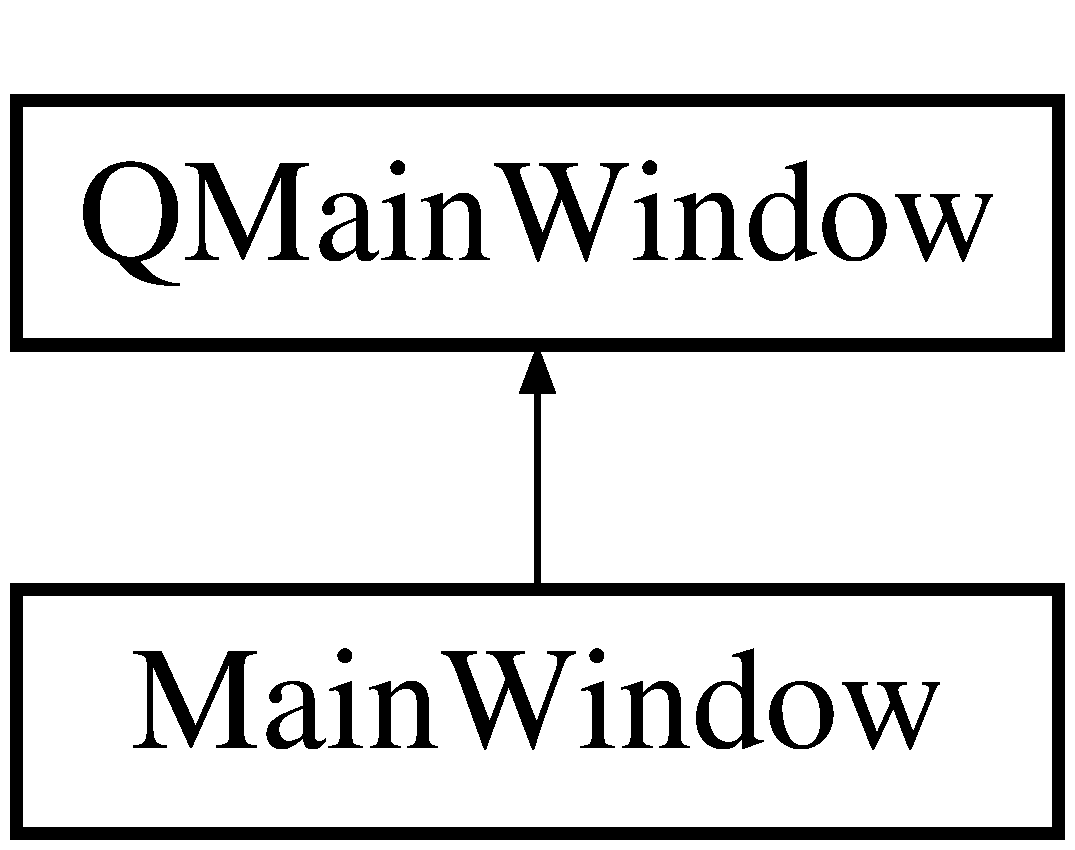
\includegraphics[height=2.000000cm]{classMainWindow}
\end{center}
\end{figure}
\subsection*{Public Slots}
\begin{DoxyCompactItemize}
\item 
\hypertarget{classMainWindow_aa3aa0f3ce42e748b931d6211921ea197}{void {\bfseries show\-About} ()}\label{classMainWindow_aa3aa0f3ce42e748b931d6211921ea197}

\item 
\hypertarget{classMainWindow_a773143409d99d112188100e1c32cb05c}{void {\bfseries go\-To\-Homepage} ()}\label{classMainWindow_a773143409d99d112188100e1c32cb05c}

\item 
\hypertarget{classMainWindow_a0acff490b8462a28cbe7627520559626}{void {\bfseries save\-Image} ()}\label{classMainWindow_a0acff490b8462a28cbe7627520559626}

\item 
\hypertarget{classMainWindow_a422893a79887001fc3eea93795593684}{void {\bfseries on\-State\-Change} ()}\label{classMainWindow_a422893a79887001fc3eea93795593684}

\item 
\hypertarget{classMainWindow_a5d6ccbf2b3dd52967400aa85207df690}{void {\bfseries on\-Engine\-Toggle} ()}\label{classMainWindow_a5d6ccbf2b3dd52967400aa85207df690}

\item 
\hypertarget{classMainWindow_a41395b3febf4c123816a19157633baaf}{void {\bfseries about\-To\-Quit} ()}\label{classMainWindow_a41395b3febf4c123816a19157633baaf}

\end{DoxyCompactItemize}
\subsection*{Public Member Functions}
\begin{DoxyCompactItemize}
\item 
\hypertarget{classMainWindow_a8b244be8b7b7db1b08de2a2acb9409db}{{\bfseries Main\-Window} (Q\-Widget $\ast$parent=0)}\label{classMainWindow_a8b244be8b7b7db1b08de2a2acb9409db}

\item 
\hypertarget{classMainWindow_a8f8abba152c87470c2c539a30a836abe}{void {\bfseries center\-And\-Resize} ()}\label{classMainWindow_a8f8abba152c87470c2c539a30a836abe}

\end{DoxyCompactItemize}


The documentation for this class was generated from the following files\-:\begin{DoxyCompactItemize}
\item 
main\-\_\-window.\-h\item 
main\-\_\-window.\-cpp\end{DoxyCompactItemize}

\hypertarget{classchess_1_1Move}{\section{chess\-:\-:Move Class Reference}
\label{classchess_1_1Move}\index{chess\-::\-Move@{chess\-::\-Move}}
}
\subsection*{Public Member Functions}
\begin{DoxyCompactItemize}
\item 
\hypertarget{classchess_1_1Move_a72979236310a7c8638ce163d8a140341}{\hyperlink{classchess_1_1Move_a72979236310a7c8638ce163d8a140341}{Move} ()}\label{classchess_1_1Move_a72979236310a7c8638ce163d8a140341}

\begin{DoxyCompactList}\small\item\em \hyperlink{classchess_1_1Move}{Move} creates a null move. \end{DoxyCompactList}\item 
\hyperlink{classchess_1_1Move_ae9a0a49737f36d5bcc6f0a80e7b6ae99}{Move} (uint8\-\_\-t from, uint8\-\_\-t to)
\begin{DoxyCompactList}\small\item\em \hyperlink{classchess_1_1Move}{Move} creates move, supplied parameters in internal board coordinate format, i.\-e. in range 21...98. \end{DoxyCompactList}\item 
\hypertarget{classchess_1_1Move_a1298f3f0cd28e307cd79ffe0555f890c}{{\bfseries Move} (uint8\-\_\-t from, uint8\-\_\-t to, uint8\-\_\-t promotion\-\_\-piece)}\label{classchess_1_1Move_a1298f3f0cd28e307cd79ffe0555f890c}

\item 
\hypertarget{classchess_1_1Move_aa1a208ecf98dc32c4dfa1b585d640045}{{\bfseries Move} (uint8\-\_\-t from, uint8\-\_\-t to, bool en\-\_\-passent)}\label{classchess_1_1Move_aa1a208ecf98dc32c4dfa1b585d640045}

\item 
\hyperlink{classchess_1_1Move_a46cebe775f30d4a02fbbcfbf1d1547ec}{Move} (Q\-String \hyperlink{classchess_1_1Move_a808b107f197231153d98d10251d9096e}{uci})
\begin{DoxyCompactList}\small\item\em \hyperlink{classchess_1_1Move}{Move} creates move from uci string (e.\-g. g1f3, d7d8\-Q etc.) \end{DoxyCompactList}\item 
\hypertarget{classchess_1_1Move_a0be2b00f7d600057abd837af8e733bd9}{{\bfseries Move} (const \hyperlink{classchess_1_1Move}{Move} \&m)}\label{classchess_1_1Move_a0be2b00f7d600057abd837af8e733bd9}

\item 
Q\-String \hyperlink{classchess_1_1Move_a808b107f197231153d98d10251d9096e}{uci} ()
\begin{DoxyCompactList}\small\item\em uci get uci string (e.\-g. g1f3, d7d8\-Q etc.) of current move \end{DoxyCompactList}\item 
\hypertarget{classchess_1_1Move_aafc06139dc4aa8ab46cd7edd0bfb44dd}{bool {\bfseries operator==} (const \hyperlink{classchess_1_1Move}{Move} \&other) const }\label{classchess_1_1Move_aafc06139dc4aa8ab46cd7edd0bfb44dd}

\item 
\hypertarget{classchess_1_1Move_a9578fdf68e54b3e3f645c06193e284e5}{bool {\bfseries operator!=} (const \hyperlink{classchess_1_1Move}{Move} \&other) const }\label{classchess_1_1Move_a9578fdf68e54b3e3f645c06193e284e5}

\end{DoxyCompactItemize}
\subsection*{Public Attributes}
\begin{DoxyCompactItemize}
\item 
\hypertarget{classchess_1_1Move_a8f8469b837fff9baad07e0dd572bbb1b}{uint8\-\_\-t {\bfseries from}}\label{classchess_1_1Move_a8f8469b837fff9baad07e0dd572bbb1b}

\item 
\hypertarget{classchess_1_1Move_a0a754e25cda786475b39e8d53a484740}{uint8\-\_\-t {\bfseries to}}\label{classchess_1_1Move_a0a754e25cda786475b39e8d53a484740}

\item 
\hypertarget{classchess_1_1Move_a7ebe3729053a5a9db82f4d74564cb7dc}{uint8\-\_\-t {\bfseries promotion\-\_\-piece}}\label{classchess_1_1Move_a7ebe3729053a5a9db82f4d74564cb7dc}

\item 
\hypertarget{classchess_1_1Move_ae69eda740543725180831fb5f76ea87d}{Q\-String {\bfseries uci\-\_\-string}}\label{classchess_1_1Move_ae69eda740543725180831fb5f76ea87d}

\item 
\hypertarget{classchess_1_1Move_a7eed53bc8f23dedc3baf77f66c57b2e6}{bool {\bfseries is\-\_\-null}}\label{classchess_1_1Move_a7eed53bc8f23dedc3baf77f66c57b2e6}

\end{DoxyCompactItemize}
\subsection*{Friends}
\begin{DoxyCompactItemize}
\item 
std\-::ostream \& \hyperlink{classchess_1_1Move_a390a2a6cfc5460a906a7d5861fd9374f}{operator$<$$<$} (std\-::ostream \&strm, const \hyperlink{classchess_1_1Move}{Move} \&m)
\begin{DoxyCompactList}\small\item\em operator $<$$<$ \end{DoxyCompactList}\end{DoxyCompactItemize}


\subsection{Constructor \& Destructor Documentation}
\hypertarget{classchess_1_1Move_ae9a0a49737f36d5bcc6f0a80e7b6ae99}{\index{chess\-::\-Move@{chess\-::\-Move}!Move@{Move}}
\index{Move@{Move}!chess::Move@{chess\-::\-Move}}
\subsubsection[{Move}]{\setlength{\rightskip}{0pt plus 5cm}chess\-::\-Move\-::\-Move (
\begin{DoxyParamCaption}
\item[{uint8\-\_\-t}]{from, }
\item[{uint8\-\_\-t}]{to}
\end{DoxyParamCaption}
)}}\label{classchess_1_1Move_ae9a0a49737f36d5bcc6f0a80e7b6ae99}


\hyperlink{classchess_1_1Move}{Move} creates move, supplied parameters in internal board coordinate format, i.\-e. in range 21...98. 


\begin{DoxyParams}{Parameters}
{\em from} & \\
\hline
{\em to} & \\
\hline
\end{DoxyParams}
\hypertarget{classchess_1_1Move_a46cebe775f30d4a02fbbcfbf1d1547ec}{\index{chess\-::\-Move@{chess\-::\-Move}!Move@{Move}}
\index{Move@{Move}!chess::Move@{chess\-::\-Move}}
\subsubsection[{Move}]{\setlength{\rightskip}{0pt plus 5cm}chess\-::\-Move\-::\-Move (
\begin{DoxyParamCaption}
\item[{Q\-String}]{uci}
\end{DoxyParamCaption}
)}}\label{classchess_1_1Move_a46cebe775f30d4a02fbbcfbf1d1547ec}


\hyperlink{classchess_1_1Move}{Move} creates move from uci string (e.\-g. g1f3, d7d8\-Q etc.) 


\begin{DoxyParams}{Parameters}
{\em uci} & supplied uci string \\
\hline
\end{DoxyParams}


\subsection{Member Function Documentation}
\hypertarget{classchess_1_1Move_a808b107f197231153d98d10251d9096e}{\index{chess\-::\-Move@{chess\-::\-Move}!uci@{uci}}
\index{uci@{uci}!chess::Move@{chess\-::\-Move}}
\subsubsection[{uci}]{\setlength{\rightskip}{0pt plus 5cm}Q\-String chess\-::\-Move\-::uci (
\begin{DoxyParamCaption}
{}
\end{DoxyParamCaption}
)}}\label{classchess_1_1Move_a808b107f197231153d98d10251d9096e}


uci get uci string (e.\-g. g1f3, d7d8\-Q etc.) of current move 

\begin{DoxyReturn}{Returns}

\end{DoxyReturn}


\subsection{Friends And Related Function Documentation}
\hypertarget{classchess_1_1Move_a390a2a6cfc5460a906a7d5861fd9374f}{\index{chess\-::\-Move@{chess\-::\-Move}!operator$<$$<$@{operator$<$$<$}}
\index{operator$<$$<$@{operator$<$$<$}!chess::Move@{chess\-::\-Move}}
\subsubsection[{operator$<$$<$}]{\setlength{\rightskip}{0pt plus 5cm}std\-::ostream\& operator$<$$<$ (
\begin{DoxyParamCaption}
\item[{std\-::ostream \&}]{strm, }
\item[{const {\bf Move} \&}]{m}
\end{DoxyParamCaption}
)\hspace{0.3cm}{\ttfamily [friend]}}}\label{classchess_1_1Move_a390a2a6cfc5460a906a7d5861fd9374f}


operator $<$$<$ 


\begin{DoxyParams}{Parameters}
{\em strm} & \\
\hline
{\em m} & \\
\hline
\end{DoxyParams}
\begin{DoxyReturn}{Returns}

\end{DoxyReturn}
prints move as uci string

Example\-: \hyperlink{classchess_1_1Move}{Move} m = \hyperlink{classchess_1_1Move}{Move}(\char`\"{}g1f3\char`\"{}); std\-::cout $<$$<$ m $<$$<$ std\-::endl; 

The documentation for this class was generated from the following files\-:\begin{DoxyCompactItemize}
\item 
chess/move.\-h\item 
chess/move.\-cpp\end{DoxyCompactItemize}

\hypertarget{classchess_1_1PgnPrinter}{\section{chess\-:\-:Pgn\-Printer Class Reference}
\label{classchess_1_1PgnPrinter}\index{chess\-::\-Pgn\-Printer@{chess\-::\-Pgn\-Printer}}
}
\subsection*{Public Member Functions}
\begin{DoxyCompactItemize}
\item 
\hypertarget{classchess_1_1PgnPrinter_a7d6e8483b5cbb4452bfa68baa0378b28}{Q\-String\-List $\ast$ {\bfseries print\-Game} (\hyperlink{classchess_1_1Game}{Game} $\ast$g)}\label{classchess_1_1PgnPrinter_a7d6e8483b5cbb4452bfa68baa0378b28}

\item 
\hypertarget{classchess_1_1PgnPrinter_a764ed0214418e2fbab5fe6f3b499e573}{void {\bfseries write\-Game} (\hyperlink{classchess_1_1Game}{Game} $\ast$g, const Q\-String \&filename)}\label{classchess_1_1PgnPrinter_a764ed0214418e2fbab5fe6f3b499e573}

\end{DoxyCompactItemize}


The documentation for this class was generated from the following files\-:\begin{DoxyCompactItemize}
\item 
chess/pgn\-\_\-printer.\-h\item 
chess/pgn\-\_\-printer.\-cpp\end{DoxyCompactItemize}

\hypertarget{classchess_1_1PgnReader}{\section{chess\-:\-:Pgn\-Reader Class Reference}
\label{classchess_1_1PgnReader}\index{chess\-::\-Pgn\-Reader@{chess\-::\-Pgn\-Reader}}
}
\subsection*{Public Member Functions}
\begin{DoxyCompactItemize}
\item 
\hypertarget{classchess_1_1PgnReader_a2ef648d6c122054f2495a48048de34fa}{\hyperlink{classchess_1_1Game}{Game} $\ast$ {\bfseries read\-Game\-From\-File} (const Q\-String \&filename)}\label{classchess_1_1PgnReader_a2ef648d6c122054f2495a48048de34fa}

\item 
\hypertarget{classchess_1_1PgnReader_a61b0f0f768fda08f1e55679ae0752b44}{\hyperlink{classchess_1_1Game}{Game} $\ast$ {\bfseries read\-Game\-From\-File} (const Q\-String \&filename, qint64 offset)}\label{classchess_1_1PgnReader_a61b0f0f768fda08f1e55679ae0752b44}

\item 
\hypertarget{classchess_1_1PgnReader_aaabd3a75f603921f6863c0c3da64901e}{Q\-String $\ast$ {\bfseries read\-File\-Into\-String} (const Q\-String \&filename)}\label{classchess_1_1PgnReader_aaabd3a75f603921f6863c0c3da64901e}

\item 
\hypertarget{classchess_1_1PgnReader_a67c553532b952f50b01efd8717694420}{\hyperlink{classchess_1_1Game}{Game} $\ast$ {\bfseries read\-Game\-From\-String} (Q\-String $\ast$pgn\-\_\-string)}\label{classchess_1_1PgnReader_a67c553532b952f50b01efd8717694420}

\item 
\hypertarget{classchess_1_1PgnReader_af66c9d84f1d0c8fe6ff8961dcd70a94b}{\hyperlink{classchess_1_1Game}{Game} $\ast$ {\bfseries read\-Game\-From\-String} (Q\-String $\ast$pgn\-\_\-string, quint64 offset)}\label{classchess_1_1PgnReader_af66c9d84f1d0c8fe6ff8961dcd70a94b}

\item 
\hypertarget{classchess_1_1PgnReader_af3852fca57fac1a7cdb223990a9b0c07}{\hyperlink{classchess_1_1Game}{Game} $\ast$ {\bfseries read\-Game} (Q\-Text\-Stream \&in)}\label{classchess_1_1PgnReader_af3852fca57fac1a7cdb223990a9b0c07}

\item 
\hypertarget{classchess_1_1PgnReader_ad60589467dafb5fb1c70d3486fd56769}{Q\-List$<$ \hyperlink{structchess_1_1HeaderOffset}{Header\-Offset} $\ast$ $>$ $\ast$ {\bfseries scan\-\_\-headers} (const Q\-String \&filename)}\label{classchess_1_1PgnReader_ad60589467dafb5fb1c70d3486fd56769}

\item 
\hypertarget{classchess_1_1PgnReader_ad7b5586d16e1922a186d1b10c3416187}{Q\-List$<$ \hyperlink{structchess_1_1HeaderOffset}{Header\-Offset} $\ast$ $>$ $\ast$ {\bfseries scan\-\_\-headers\-From\-String} (Q\-String $\ast$content)}\label{classchess_1_1PgnReader_ad7b5586d16e1922a186d1b10c3416187}

\end{DoxyCompactItemize}


The documentation for this class was generated from the following files\-:\begin{DoxyCompactItemize}
\item 
chess/pgn\-\_\-reader.\-h\item 
chess/pgn\-\_\-reader.\-cpp\end{DoxyCompactItemize}

%--- End generated contents ---

% Index
\newpage
\phantomsection
\addcontentsline{toc}{chapter}{Index}
\printindex

\end{document}
